% \documentclass[review]{elsarticle}
\documentclass[utf8, babel, sor, jor, amsmath, amssymb, reprint]{elsarticle} %удалить перед отправкой
\graphicspath{{images/}}

\usepackage{lineno,hyperref}
\usepackage{algorithm}
\usepackage{algorithmic}
\modulolinenumbers[5]

\journal{Physica A: Statistical Mechanics and its Applications}

\bibliographystyle{elsarticle-num}

\usepackage{mathrsfs}
\usepackage{amsmath}
\usepackage{amssymb}%
\usepackage{multirow}



%%%%%%%%%%%%%%%%%%%%%%%
%% Elsevier bibliography styles
%%%%%%%%%%%%%%%%%%%%%%%
%% To change the style, put a % in front of the second line of the current style and
%% remove the % from the second line of the style you would like to use.
%%%%%%%%%%%%%%%%%%%%%%%

%% Numbered
%\bibliographystyle{model1-num-names}

%% Numbered without titles
%\bibliographystyle{model1a-num-names}

%% Harvard
%\bibliographystyle{model2-names.bst}\biboptions{authoryear}

%% Vancouver numbered
%\usepackage{numcompress}\bibliographystyle{model3-num-names}

%% Vancouver name/year
%\usepackage{numcompress}\bibliographystyle{model4-names}\biboptions{authoryear}

%% APA style
%\bibliographystyle{model5-names}\biboptions{authoryear}

%% AMA style
%\usepackage{numcompress}\bibliographystyle{model6-num-names}

%% `Elsevier LaTeX' style
\bibliographystyle{elsarticle-num}
%%%%%%%%%%%%%%%%%%%%%%%


\usepackage{xcolor}
\newcommand{\todo}[1] {\textcolor{red}{#1}} %%for TODO comments
\def\l{\left\langle}
\def\r{\right\rangle}
\usepackage{mathrsfs}
\usepackage{amsmath}
\usepackage{amssymb}%

\begin{document}

\begin{frontmatter}


\title{Nature of frustrations in the ground state of the $\pm J$ Ising model on a square lattice}

\author[mainaddress, secondaryaddress]{Viacheslav Trukhin\corref{mycorrespondingauthor}}
\ead{trukhin.vo@dvfu.ru}

\author[mainaddress]{Egor Prokhorov\corref{mycorrespondingauthor}}
\ead{prokhorov.ei@dvfu.ru}

\author[mainaddress, secondaryaddress]{Aleksandr Makarov\corref{mycorrespondingauthor}}
\ead{makarov.ag@dvfu.ru}

\author[mainaddress, secondaryaddress]{Konstantin Nefedev\corref{mycorrespondingauthor}}
\ead{nefedev.kv@dvfu.ru}


\address[mainaddress]{Far Eastern Federal University, Vladivostok, Russky Island, 10 Ajax Bay, 690922, the Russian Federation}
\address[secondaryaddress]{Institute of Applied Mathematics, Far Eastern Branch, Russian Academy of Science, Vladivostok, Radio 7, 690041, the Russian Federation}

\begin{abstract}

By the complete enumeration method, all possible states of the Edwards-Anderson model on a simple square lattice of $8 \times 8$ spins were accurately calculated. The ground-state energy for the studied finite-size samples was determined. The macroscopic degeneracy of the ground state in frustrated spin systems is due to the combinatorics of frustrated plaquettes, i.e., the number of ways to place frustrated spin pairs on the lattice. The algorithm for calculating energy, spin excess, and ground-state configurations is based on identifying the arrangement of frustrations. The dependence of the ground-state spin excess in the Edwards-Anderson model on an external magnetic field has a discrete (step-like, stair-like) character. Critical values of the external magnetic field at which large jumps in residual entropy, were calculated. The nature of these large entropy jumps is explained by the fact that at certain critical values of the external magnetic field, the sum of several spin configurations with different interaction energies and Zeeman energies, i.e., with different values of spin excess, will have the same total energy. The degeneracy multiplicities of states with the same total energy are summed up at the critical value of magnetic field.

\end{abstract}


\begin{highlights}  
	\item The presence of frustrations in the ground state does not necessarily lead to macroscopic degeneracy.  
	\item The effect of finite-size scaling on the entropy and energy of the ground state has been accurately computed, and the asymptotic behavior of the residual entropy has been determined.  
	\item The phenomenon of macroscopic degeneracy of the ground state is due to the arrangement of frustrated plaquettes in the lattice.  
	\item The spin excess in the ground state is determined by the lattice phase.  
\end{highlights}  


\begin{keyword}
	Ising model, Ground state, GPU and CPU high performance calculations, statistical thermodynamics.
\end{keyword}


\end{frontmatter}

\linenumbers

\newpage
\tableofcontents

\newpage
\section{Introduction}

Without exaggeration, solving models of frustrated systems, such as spin glasses and spin ice, is one of the most important research areas in statistical mechanics. The Edwards-Anderson (EA) Ising spin glass model is one of the simplest spin glass models with short-range interactions \cite{edwards1975theory}. Despite its apparent simplicity, the low-temperature properties of this model, even in 2D and especially in higher dimensions, remain poorly understood \cite{pal1996ground, hartmann2011ground, newman2022ground}. Spin lattice models with competing ferromagnetic and antiferromagnetic interactions have been studied for many years \cite{binder1986spin, mezard1987spin, lebrecht2004plaquette, valdes2012j, lebrecht2015j, fan2023searching}.

Despite many years of intensive research, the nature of the low-temperature phase of the Ising model for frustrated spin systems with a limited interaction range remains unresolved \cite{roma2010ground, newman2023proof}. Two of the most important open questions concern the properties of the ground state of spin glasses (i.e., at zero temperature), particularly the degeneracy of the ground state and the nature of low-energy excitations \cite{newman2022ground}.

The calculation of the energy, entropy, and spin excess of the ground state of a spin glass with a given Hamiltonian, even without an external magnetic field, is a highly complex optimization problem. In three dimensions, this problem is $NP$-hard \cite{barahona1982computational, hartmann2002optimization}, meaning that no known algorithm can solve the problem of spin excess, energy, and ground-state degeneracy in time proportional to a polynomial function of the linear system size, and it is widely believed that such an algorithm cannot be developed. Currently, no algorithm combines high accuracy with efficiency \cite{fan2023searching}.

The properties of spin glasses at zero temperature are typically studied using approximate methods \cite{roma2009ground, perez2012ground}. Over time, various approximate approaches for solving spin system models have been developed, but the problem remains relevant due to the lack of an exact solution \cite{rybin2022hybrid, makarova2023canonical, farias2024differentiable}. However, for some lattices, such as the triangular lattice, it is possible to obtain information about entropic and magnetic properties \cite{jurvcivsinova2024classical}.

Energy can be computed using optimization methods \cite{hartmann2002optimization, hartmann2004new}, genetic algorithms \cite{holland1992adaptation}, annealing algorithms \cite{kirkpatrick1983optimization}, multicanonical sampling methods \cite{berg1994ground, shevchenko2017multicanonical}, multi-spin cluster methods \cite{makarova2023canonical}, or parallel tempering \cite{PhysRevB.50.16444, roma2009ground}.

Entropy, or the degeneracy of the ground state, is crucial information not only for understanding the low-temperature behavior of spin glasses (or spin ice) but also for the nature of excitations. Even for the 2D Edwards-Anderson model, computing the ground state is a non-trivial problem. Approximating entropy or the degeneracy multiplicity is an even more challenging task. Methods such as the transfer matrix method \cite{PhysRevB.22.288, cheung1983equilibrium, kolan1982ground}, ballistic search \cite{hartmann2000ground}, thermodynamic integration \cite{kirkpatrick1977frustration, binder1985monte, roma2004ground}, and multicanonical sampling \cite{berg1994ground, shevchenko2017multicanonical} have been developed to address this issue. However, for finite systems with a countable number of spins, approximate methods are unlikely to be applicable.  

Spin system models on lattices provide an ideal platform for exploring complex magnetic ground states with excitations, and their investigation is important for the advancement of physics \cite{lacroix2011introduction}. This research includes determining the critical switching fields between ground states in an external magnetic field, entropy jumps during transitions between ground states, and correlation functions \cite{ramirez2004effect, rosas2004random, andriushchenko2019large}.  

Studying the energy landscape of low-energy states in spin glasses \cite{biswas2023energy} remains a pressing problem, as does research on spin ice. An intriguing question is identifying the relative fraction (or concentration) of ferromagnetic (or antiferromagnetic) exchange interactions at $T=0$ that results in a transition between ferromagnetic and spin glass states (or between antiferromagnetic and spin glass states) \cite{gruzberg2001random, honecker2001universality, picco2006strong, tsomokos2011interplay, zimmer2022role}. The thermodynamic properties and phase diagram of the ground state for molecular clusters with a small number of spins were calculated in \cite{dias2023ground}.

Ground-state configurations, as well as excitations in the ground and low-energy states of spin glasses, along with macroscopic ground-state degeneracy and residual entropy at low temperatures, are actively studied in models with long-range dipolar interactions \cite{makarova2021low, singh2024micromagnetic}. The search for spin glass ground states is not only essential for understanding the nature of disordered magnets and many other physical systems but also proves useful for solving a wide range of complex combinatorial optimization problems in various disciplines. Despite decades of effort, no algorithm with both high accuracy and efficiency has yet been developed \cite{fan2023searching}.  

Estimating the ground-state energy and understanding the nature of its macroscopic degeneracy have remained open problems for many years. At low temperatures, the spin glass in its ground state is realized solely through configurations with minimal interaction energy, while the ensemble of other configurations in the Gibbs distribution plays no role. Ground-state energies calculated by various methods in studies \cite{thouless1977solution, sherrington1975solvable, tanaka1980analytic, klein1976comparison, kirkpatrick1978infinite, karandashev2019global, palmer1999ground, campbell2004energy, roma2009ground} show significant variability.  

It will be shown below that this variability may be related to the distribution of frozen disorder in the bonds, i.e., competing ferromagnetic and antiferromagnetic interactions. For a finite number of spins, the ground-state energy strongly depends on the specific realization of the distribution $\left\lbrace J_{ij} \right\rbrace$ on the spin lattice.  

In this work, we utilized an complete enumeration algorithm \cite{dias2023ground, padalko2021parallel} to solve the problem of ground-state energy for a finite number of spins, to compute the degeneracy of this state, and to determine the distribution of spin excess. The availability of an exact solution, even for a relatively small number of spins, allows for testing approximate methods. By performing complete enumeration method, we identified all possible states, enabling us to calculate properties in the presence of an external magnetic field.

\section{Plaquette combinatorics}

Let by a plaquette we mean a closed chain of spins of minimal length \cite{lebrecht2015j}.In the following examples on a square lattice, the plaquettes are elementary squares, see Figures \ref{fig:Type1}, \ref{fig:Type2}, \ref{fig:Type3}. In the Edwards-Anderson spin glass model, the plaquettes can be classified into three possible types. 

If $P_+$ is the relative amount of ferromagnetic ($J_{ij}=+1$) exchange integrals, then Type-I, see Figure \ref{fig:Type1}, belongs to the plaquettes in which $P_+=0.5$. For Type-II, $P_+=0.75$ or $P_+=0.25$ (Figure \ref{fig:Type2}). For Type-III, $P_+=1.0$ or $P_+=0.0$ (Figure \ref{fig:Type3}). Straight and jagged lines in the figures correspond to ferromagnetic and antiferromagnetic bonds, respectively. White and black circles in the figures correspond to up and down spins in one of the ground state configurations.


\begin{figure}[H]
	\centering
	\begin{minipage}{0.3\textwidth}
		\centering
		\resizebox{45px}{45px}{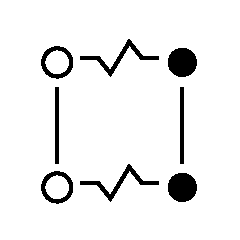
\includegraphics{pictures/Type1_1.eps}}
		\hspace{-4pt} 
		\resizebox{45px}{45px}{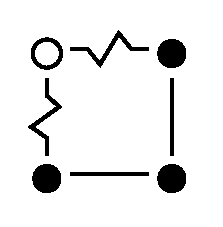
\includegraphics{pictures/Type1_2.eps}}
		\caption{Type-I plaquettes}
		\label{fig:Type1} 
	\end{minipage}
	\hspace{5pt} 
	\begin{minipage}{0.3\textwidth}
		\centering
		\resizebox{45px}{45px}{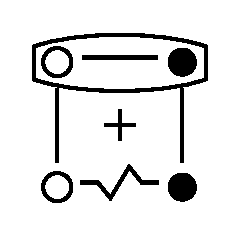
\includegraphics{pictures/Type2_1.eps}}
		\hspace{-2pt} 
		\resizebox{45px}{45px}{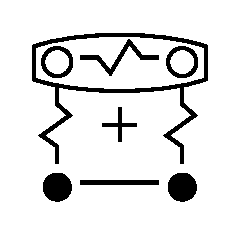
\includegraphics{pictures/Type2_2.eps}}
		\caption{Type-II plaquettes}
		\label{fig:Type2}
	\end{minipage}
	\hspace{5pt}
	\begin{minipage}{0.3\textwidth}
		\centering
		\resizebox{45px}{45px}{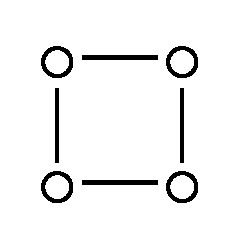
\includegraphics{pictures/Type3_1.eps}}
		\hspace{-4pt} 
		\resizebox{45px}{45px}{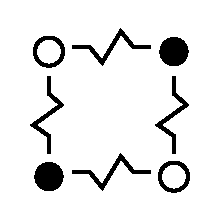
\includegraphics{pictures/Type3_2.eps}}
		\caption{Type-III plaquettes}
		\label{fig:Type3}
	\end{minipage}
\end{figure}


There are $2^4$ configurations in each of the above considered plaquettes.
It was found that frustration (excitation or positive energy of the exchange interaction between $ij$-pairs of spins) in the ground state necessarily appears in Type-II plaquettes, which are marked by the $‘+’$ sign. Moreover the frustrated pair can be any pair of spins.


If the system consists of two Type-II plaquettes, for example, as shown in Figure \ref{fig:Type2_32}, the frustrated pair is necessarily located at the intersection of the plaquettes to minimise the energy, regardless of the distribution of exchange interactions in the rest of the lattice. 

\begin{figure}[H]
	\centering
	\begin{minipage}{0.2\textwidth}
		\centering
		(a)
		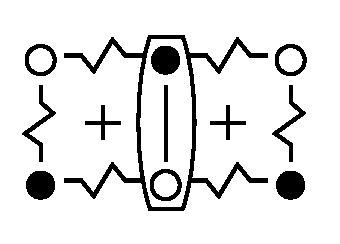
\includegraphics[width=1\textwidth]{pictures/Type2_3x2.eps}
		\label{fig:Type2_3x2}
	\end{minipage}
	\hspace{20pt}
	\begin{minipage}{0.2\textwidth}
		\centering
		(b)
		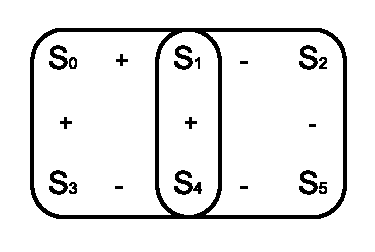
\includegraphics[width=1\textwidth]{pictures/Type2_3x2_2.eps}
		\label{fig:Type2_3x2_2}
	\end{minipage}
	\caption{Systems of two Type-II plaquettes}
	\label{fig:Type2_32}
\end{figure}


It is easy to find the energy, spin excess and configurations of the ground state at the known arrangement of frustrated pairs of spins. The energy and degeneracy multiplicity of the ground state for the systems in Figure \ref{fig:Type2_32} $E_{gs}/N=-0.83$, $g_{gs}=2$. The ground state spin excess $M_{gs}/N=0$ for the system in Figure \ref{fig:Type2_32}(a) and $M_{gs}/N=\pm 0.33$ in Figure \ref{fig:Type2_32}(b).
In Figures \ref{fig:4x4.1}(a-d), there is a Type-II plaquette containing frustration in the center of the lattice. Placing frustration in a non-Type-II plaquette results in another excitation in it. In this example, there are 8 ground states ($E_{gs}/N=-1.25$, $g_{gs}=8$, $M_{gs}/N=\pm 0.25$ - Figure \ref{fig:4x4.1}(a), $M_{gs}/N=\pm 0.25$ - Figures \ref{fig:4x4.1}(a,b), $M_{gs}/N=\pm 0.08$ - Figure \ref{fig:4x4.1}(c), $M_{gs}/N=\pm 0.08$ - Figure \ref{fig:4x4.1}(d)). The spin excess of the ground state is due to the ratio of the number of ferromagnetic to antiferromagnetic bonds. Frustrations can change this ratio because a frustrated antiferromagnetic bond will lead to ferromagnetic ordering in the spin pair, and vice versa.

\begin{figure}[H]
	\begin{minipage}[h]{0.2\linewidth}
		\centering(a)
		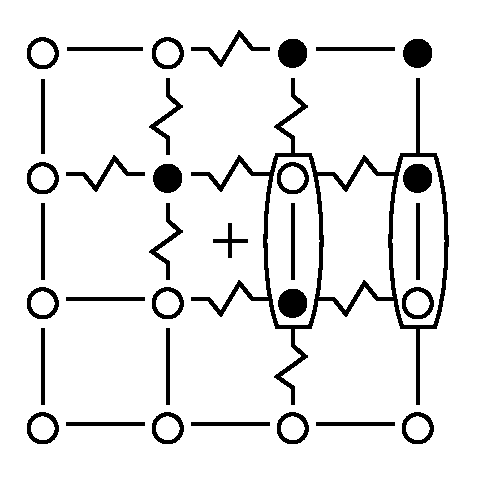
\includegraphics[width=1\linewidth]{pictures/Cl1_Type2_gs1.eps}
	\end{minipage}
	\hfill
	\begin{minipage}[h]{0.2\linewidth}
		\centering(b)
		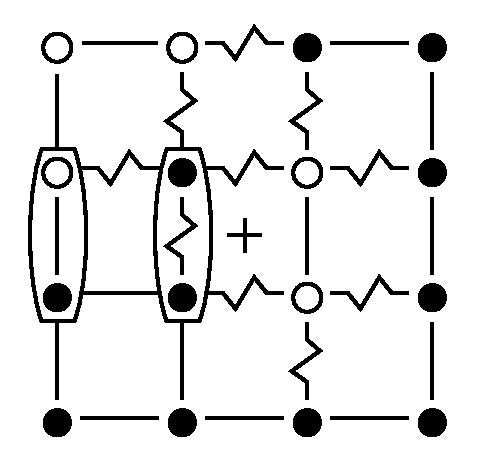
\includegraphics[width=1\linewidth]{pictures/Cl1_Type2_gs2.eps}
	\end{minipage}
	\hfill
	\begin{minipage}[h]{0.2\linewidth}
		\centering(c)
		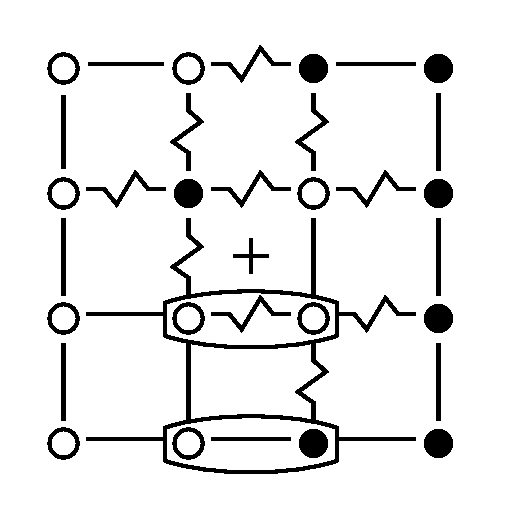
\includegraphics[width=1\linewidth]{pictures/Cl1_Type2_gs3.eps}
	\end{minipage}
	\hfill
	\begin{minipage}[h]{0.2\linewidth}
		\centering(d)
		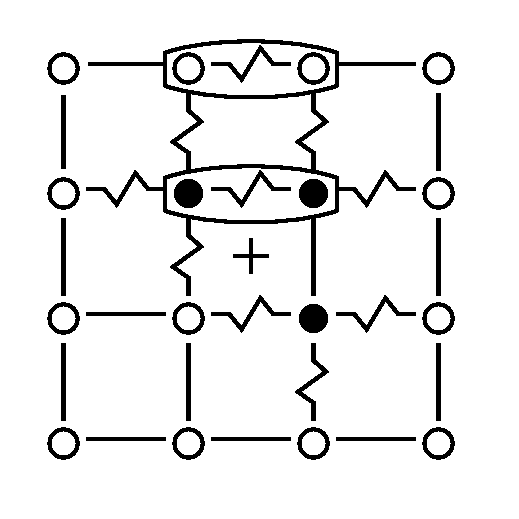
\includegraphics[width=1\linewidth]{pictures/Cl1_Type2_gs4.eps}
	\end{minipage}
	\caption{The ground states of the system (a, b, c, d). Frustrated pairs of spins are circled.}
	\label{fig:4x4.1}
	
\end{figure}

For the example in Figure \ref{fig:4x7}, $E_{gs}/N=-1.18$, $M_{gs}/N=0$, there are only two ground states $g_{gs}=2$. At the same time, there are three frustrated pairs. Thus, the presence of frustrations in the ground state does not always lead to macroscopic degeneracy. 

\begin{figure}[H]
	\centering
	\resizebox{150px}{75px}{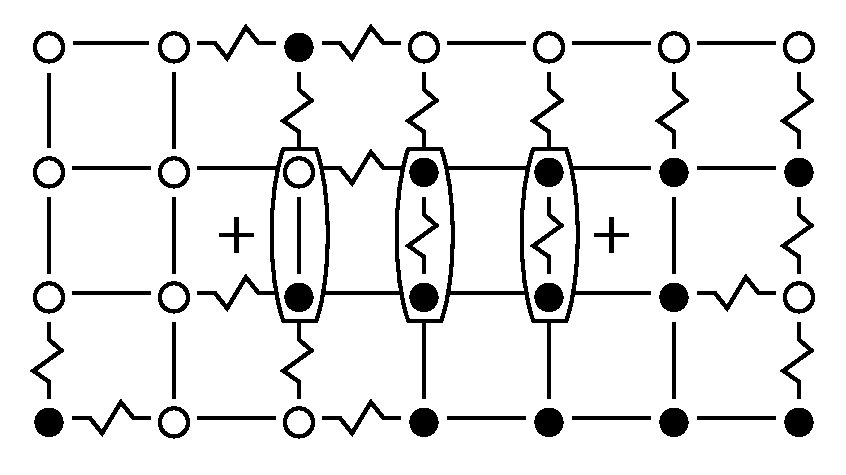
\includegraphics{pictures/Cl7x4_Type2.eps}}
	\caption{The ground state of the lattice with two Type-II plaquettes}
	\label{fig:4x7}
\end{figure}

Figure \ref{fig:5x5.22F} shows an example ($E_{gs}/N=-1.44$, $g_{gs}=4$, $M_{gs}/N=\pm 0.11$ for Figure \ref{fig:4x7}(a) and $M_{gs}=\pm 0.04$ for \ref{fig:4x7}(b)) when two Type-II plaquettes share a common spin. Despite the decrease in the number of frustrated pairs, there is an increase in the ground state degeneracy compared to the previous example. The combinatorics arises because there are several options for the placement of frustrated pairs on the lattice.

\begin{figure}[H]
	\centering
	\begin{minipage}[h]{0.25\linewidth}
		\centering(a)
		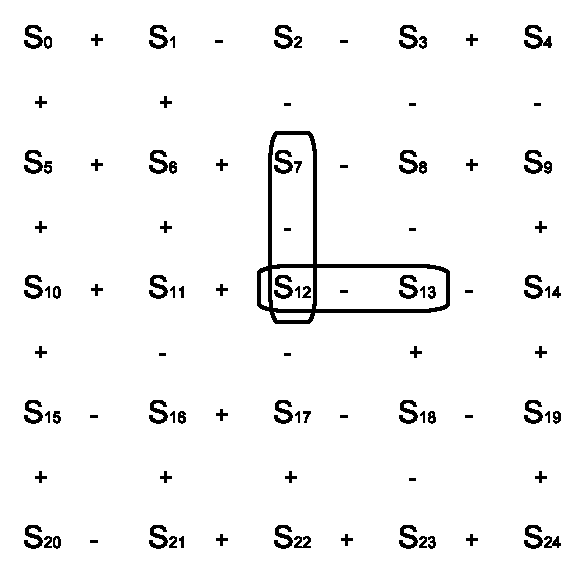
\includegraphics[width=1\linewidth]{pictures/Cl5x5_Type2_gs1.eps}
	\end{minipage}
	\hspace{15pt}
	\begin{minipage}[h]{0.25\linewidth}
		\centering(b)
		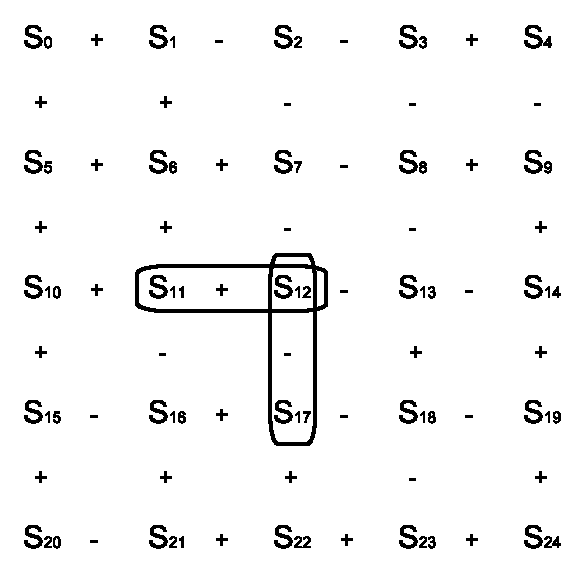
\includegraphics[width=1\linewidth]{pictures/Cl5x5_Type2_gs2.eps}
	\end{minipage}
	\caption{Ground states of the lattice with two Type-II plaquettes}
	\label{fig:5x5.22F}
\end{figure}

Several conclusions can be drawn from the examples discussed:

\begin{enumerate}
	\item Type-II plaquettes are the only cause of frustrations in the ground state.
	\item In the ground state, frustrations are located between Type-II plaquettes or between a plaquette and the edge of the grid, depending on the distances.
	\item Macroscopic degeneration of the ground state is due to alternative frustration locations.
\end{enumerate}

\section{Nature of the ground state degeneracy}

It is possible to calculate all ground states by pairwise combination of Type-II plaquettes. Let us consider the operation of the algorithm on the example of a lattice consisting of 64 spins \ref{fig:12PS_cell64_J72_5}(a).

\begin{figure}[H]
	\centering
	\begin{minipage}[h]{0.3\linewidth}
		\centering(a)
		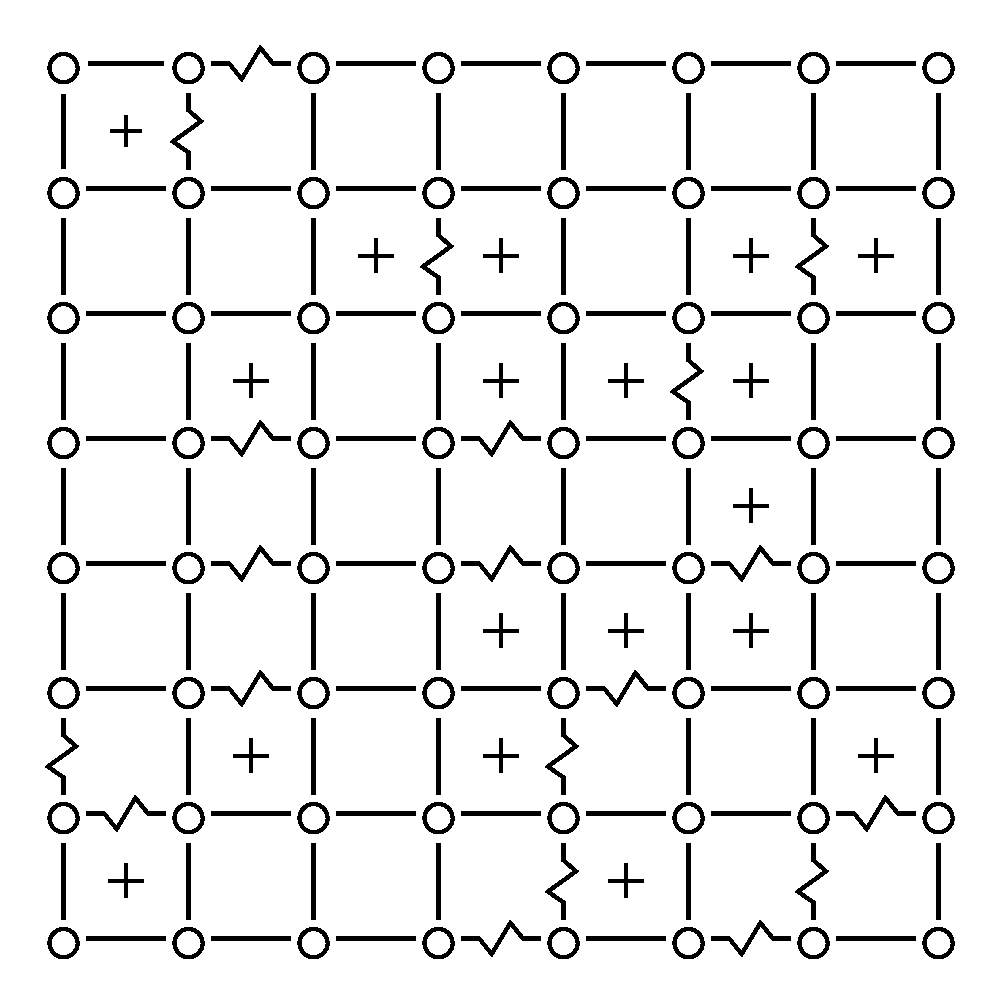
\includegraphics[width=1\linewidth]{pictures/cell64_J72_5.eps}
	\end{minipage}
	\hspace{10pt}
	\begin{minipage}[h]{0.3\linewidth}
		\centering(b)
		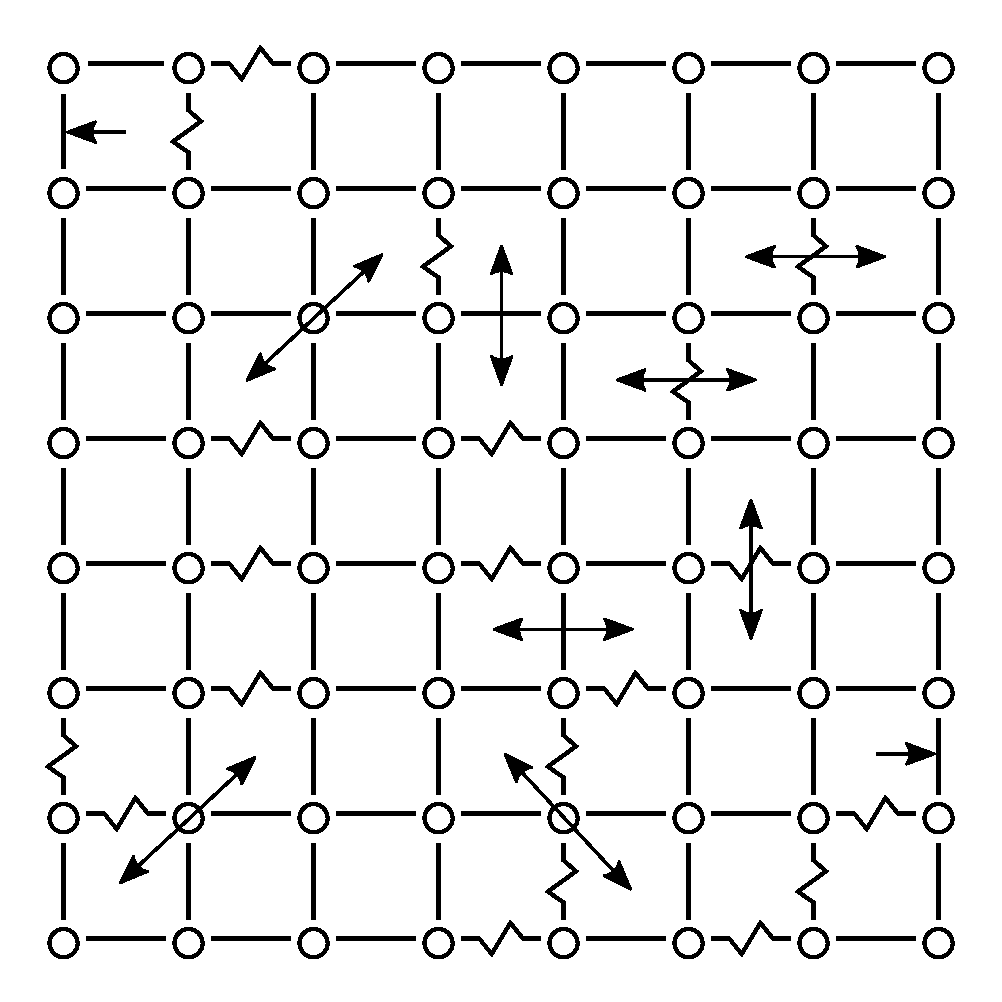
\includegraphics[width=1\linewidth]{pictures/1PS_cell64_J72_5.eps}
	\end{minipage}
	\hspace{10pt}
	\begin{minipage}[h]{0.3\linewidth}
		\centering(c)
		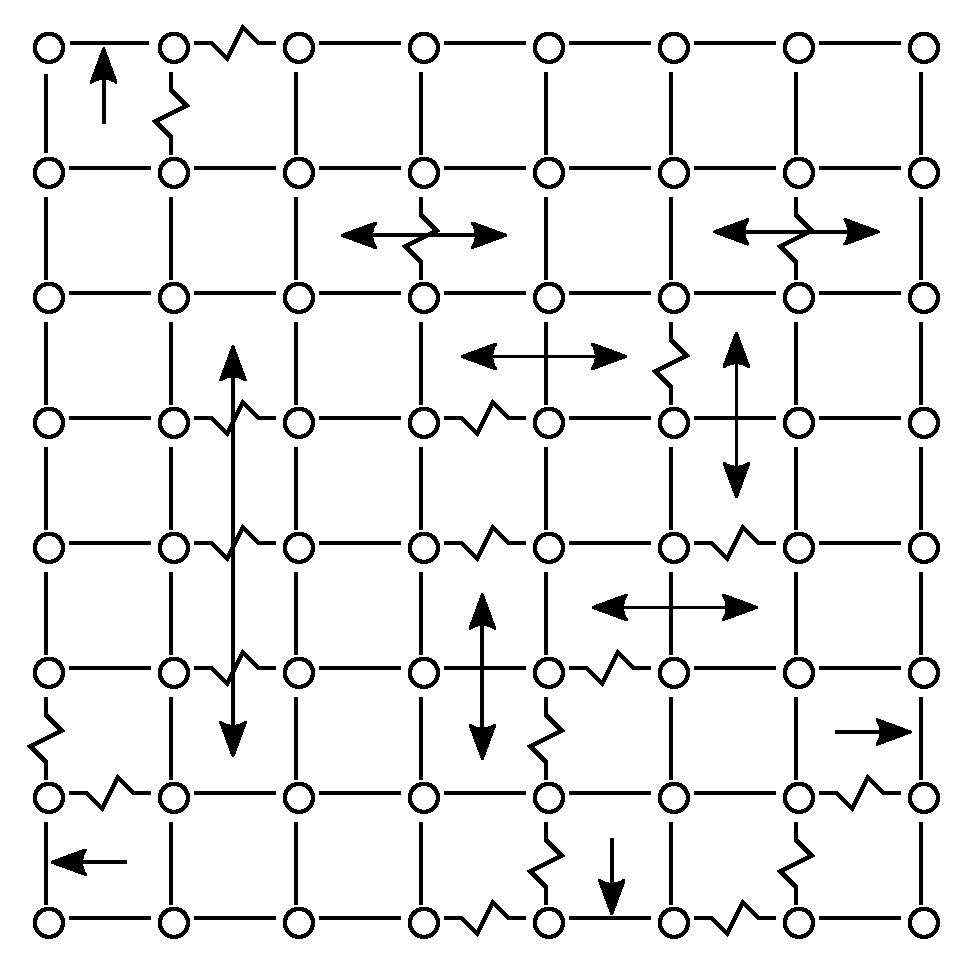
\includegraphics[width=1\linewidth]{pictures/2PS_cell64_J72_5.eps}
	\end{minipage}
	\caption{(a) - an example of a lattice with 64 spins, (b, c) - combinations of Type-II plaquettes with the minimal number of frustrations}
	\label{fig:12PS_cell64_J72_5}
\end{figure}


First, each plaquette is assigned coordinates $x$ and $y$. Next, the partitioning of the Type-II plaquettes into pairs is combined. We consider the cases when frustrations occur between each pair of plaquettes and when the placement of excitations occurs between a plaquette and the edge of the lattice.The number of frustrations between $i,j$-th pair of plaquettes is defined as $\left|x_i-x_j\right|+\left|y_i-y_j\right|$, the number of frustrations occurring from the Type-II plaquette to the nearest edge of the grid is defined as $R_{ij}+1$, where $i$ is the number of the Type-II plaquette, $j$ is the number of the nearest plaquette on the edge of the grid, $R_{ij}$ is the distance between them. After enumerating all pairs of Type-II plaquettes, the combinations that are calculated to have the minimum number of frustrations are considered. Two of them are shown in Figure \ref{fig:12PS_cell64_J72_5}(b,c).

Based on the combinations obtained, the spin pairs between the plaquettes are marked as frustrated (Figure \ref{fig:12F_cell64_J72_5}).

\begin{figure}[H]
	\centering
	\begin{minipage}[h]{0.3\linewidth}
		\centering(a)
		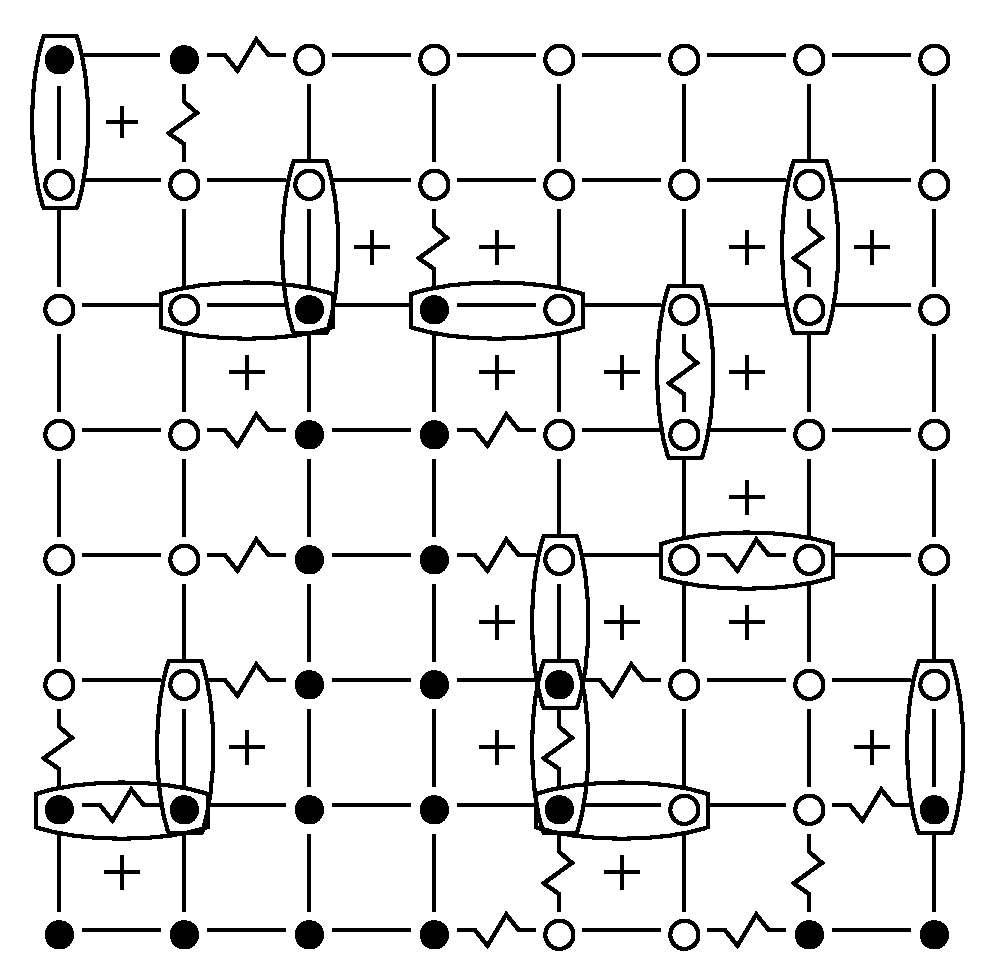
\includegraphics[width=1\linewidth]{pictures/1Conf_cell64_J72_5.eps}
	\end{minipage}
	\hspace{15pt}
	\begin{minipage}[h]{0.3\linewidth}
		\centering(b)
		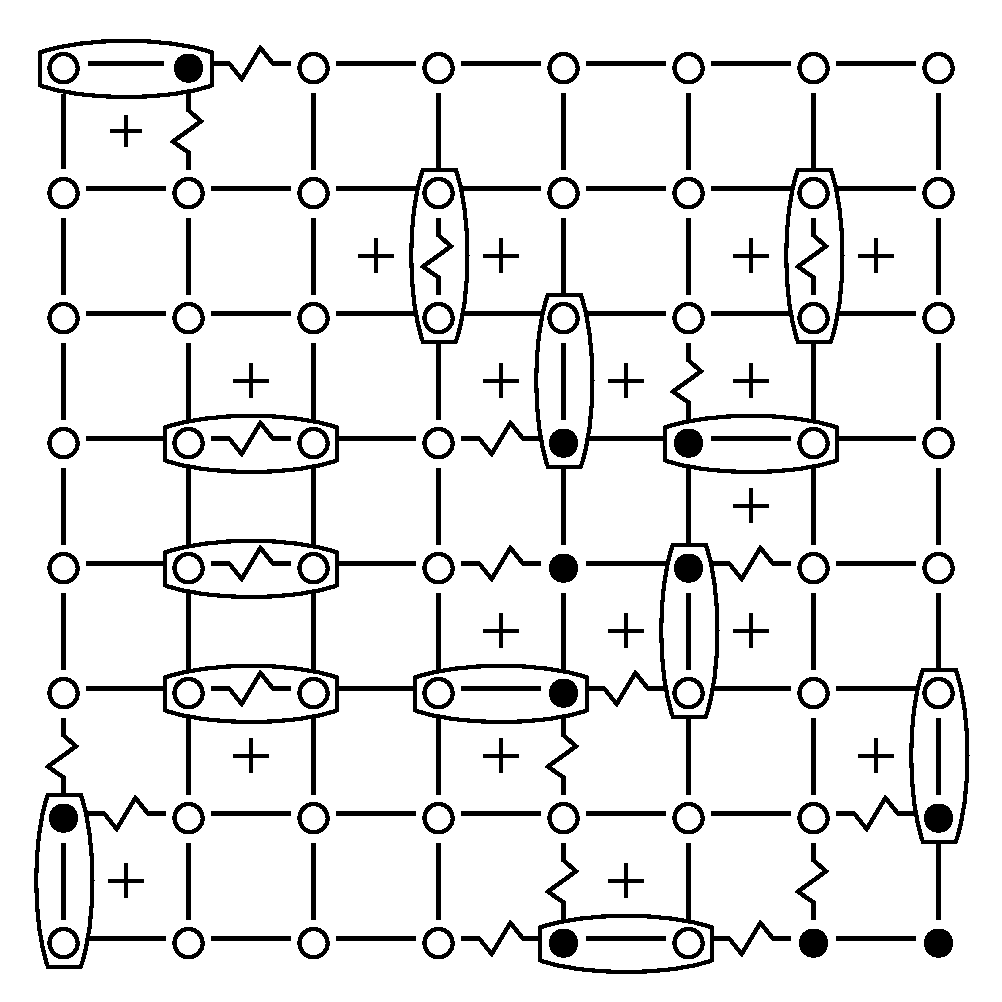
\includegraphics[width=1\linewidth]{pictures/2Conf_cell64_J72_5.eps}
	\end{minipage}
	\caption{Ground states of the lattice\ref{fig:12PS_cell64_J72_5}(a)}
	\label{fig:12F_cell64_J72_5}
\end{figure}

In total, $g_{gs}=124$ ground states with energy $E_{gs}/N=-1.34$ and spin excess $M_{gs}/N$ from $\pm 0.28$ to $\pm 0.66$ were obtained for this lattice. This solution is in good agreement with the results obtained with the algorithm \ref{alg:addititional_algorithm}.

Thus, the high multiplicity of the ground state degeneracy is due to several reasons:

\begin{enumerate}
	\item Different combinations of Type-II plaquettes can produce the same number of frustrations, as shown in the previous example in Figures \ref{fig:12PS_cell64_J72_5}(b,c).
	\item There may be several options for placing frustrations between plaquettes if their $x,y$ coordinates are different (Figure \ref{fig:5x5.22F}).
	\item The choice of boundary conditions can affect degeneracy. For example, in the case of placing a frustrated plaquette next to two boundaries leads to an increase in frustration choices (Figure \ref{fig:4x4.1}).
\end{enumerate}

\section{Complete enumeration solution}

To investigate the problem, an complete enumeration algorithm was developed.
The Edwards-Anderson spin glass model is represented by a 2D Ising lattice:

\begin{equation}
	E = -\sum J_{ij} S_i S_j + h \sum S_i.
	\label{eq:ising_energy}
\end{equation}

This results in competing antiferromagnetic (for $J_{ij} = -1$) and ferromagnetic (for $J_{ij} = +1$) interactions. In our model, the energy of exchange interactions does not depend on the distance between interacting spins. However, the alternating nature of exchange integrals $J_{ij}$ may be attributed to distortions in the arrangement of interacting atoms on the lattice or oscillations in electron density.

Let us consider a one-dimensional chain of three spins ($L = 3$) interacting ferromagnetically. Hence, all $J_{ij} = +1$. Let $\beta = (kT)^{-1}$. The partition function is given by:

\begin{equation}
	Z_3 = e^{3\beta - 3\beta h} + 3e^{\beta - h - \beta} + 3e^{\beta h - \beta} + e^{3\beta + 3\beta h}.
	\label{eq:stat_3}
\end{equation}

Now, let us attach a second chain parallel to the first one. Assuming all interactions are ferromagnetic:

\begin{equation}
	\label{eq:stat_3_un}
	\begin{alignedat}{2}
		Z_6 = Z_3 e^{\beta h-\beta} + Z_3 e^{\beta h-\beta} + Z_3 e^{\beta h-\beta} + Z_3 e^{3 \beta +3 \beta h} + \\
		Z_3 e^{-\beta h-\beta} + Z_3 e^{-\beta h-\beta} + Z_3 e^{-\beta h-\beta} + Z_3 e^{3 \beta -3 \beta h}.
	\end{alignedat}
\end{equation}

As a result, the partition function for a $3 \times 2$ lattice is:

\begin{equation}
	\label{eq:stat_3_res}
	\begin{alignedat}{2}
		Z_6 = 6 e^{-5 \beta } + 12 e^{-\beta } + 2 e^{3 \beta } + e^{9 \beta -6 \beta  h} + 6 e^{3 \beta -4 \beta  h} + 6 e^{-3 \beta -2 \beta  h} + \\
		9 e^{\beta -2 \beta  h} + 6 e^{2 \beta  h-3 \beta } + 9 e^{\beta +2 \beta  h} + 6 e^{3 \beta +4 \beta  h} + e^{9 \beta +6 \beta  h}.
	\end{alignedat}
\end{equation}

The numerical algorithm for calculating partition function parameters (state density, degeneracy or entropy, energy, and spin excess) is then outlined as follows (\ref{alg:addititional_algorithm}):

\begin{algorithm}[H]
	\textbf{INPUT:} Lattice size and geometry (number and coordinates of spins, boundary conditions, number of neighbors), distribution of exchange constants.\\
	\textbf{OUTPUT:} Partition function parameters, state density (degeneracy or entropy, energy, and spin excess).
	\begin{algorithmic}
		\STATE {Compute state density for the first 1D chain.}
		\FOR {Number of lattice layers \\}
		{
			\STATE {Compute state density for the attached 1D chain.}
			\FOR {Length of the 1D chain \\}
			{
				\STATE {Compute state density for the resulting lattice.}
			}
			\ENDFOR \\
		}
		\ENDFOR
	\end{algorithmic}
	\caption{Computing partition function parameters by attaching 1D chains.}
	\label{alg:addititional_algorithm}
\end{algorithm}

As a result, for a square lattice of size $L \times L = N$, the computational complexity of complete enumeration is reduced from $2^{N}$ to $L \cdot 2^L + (L - 1) \cdot 2^L$. Thus, the performance gain is approximately 92\% for a 9-spin lattice and spans 27 orders of magnitude for a system with 100 spins.


\section{Ground state energy}

The results of solving the problem of calculating the ground state energy of spin glass in the Edwards-Anderson model are presented in Table \ref{tab:Egs}. The table shows that the ground state energy values exhibit significant variability.

\begin{table}[h]
	\begin{tabular}{|l|c|l|}
		\hline
		Method                                   & $E_{gs}$                                       & Ref.                                          \\ \hline
		Thouless-Anderson-Palmer (TAP) Approach & 0                                              & \cite{thouless1977solution}    \\ \hline
		Replica Method                            & $-2/\pi$                                       & \cite{sherrington1975solvable} \\ \hline
		Partition function                      & -0.5                                           & \cite{tanaka1980analytic}      \\ \hline
		Mean random field                       & $-1/\sqrt{2\pi}$                               & \cite{klein1976comparison}     \\ \hline
		Monte-Carlo                             & -0.76                                          & \cite{kirkpatrick1978infinite} \\ \hline
		Algorithm of Shraudorphs-Kamensky        & -1.33                                          & \cite{karandashev2019global}   \\ \hline
		Parallel Tempering   & -1.40193                                       & \cite{palmer1999ground}        \\ \hline
		Branch-and-Cut Algorithm              & -1.40197                         
		& \cite{campbell2004energy}      \\ \hline
		
		Parallel tempering Monte-Carlo  & -1.31479                                       & \cite{roma2009ground}          \\ \hline
		
		
		
	\end{tabular}
	\caption{Ground state specific energy}
	\label{tab:Egs}
\end{table}

We calculated the ground state energy in the Edwards-Anderson model exactly using complete enumeration algorithm \ref{alg:addititional_algorithm}. The graph in Figure \ref{fig:E(Q)} shows the dependence of the specific ground state energy $E_{gs}/N$ on the number of Type-II plaquettes $Q$.

\begin{figure}[H]
	\centering
		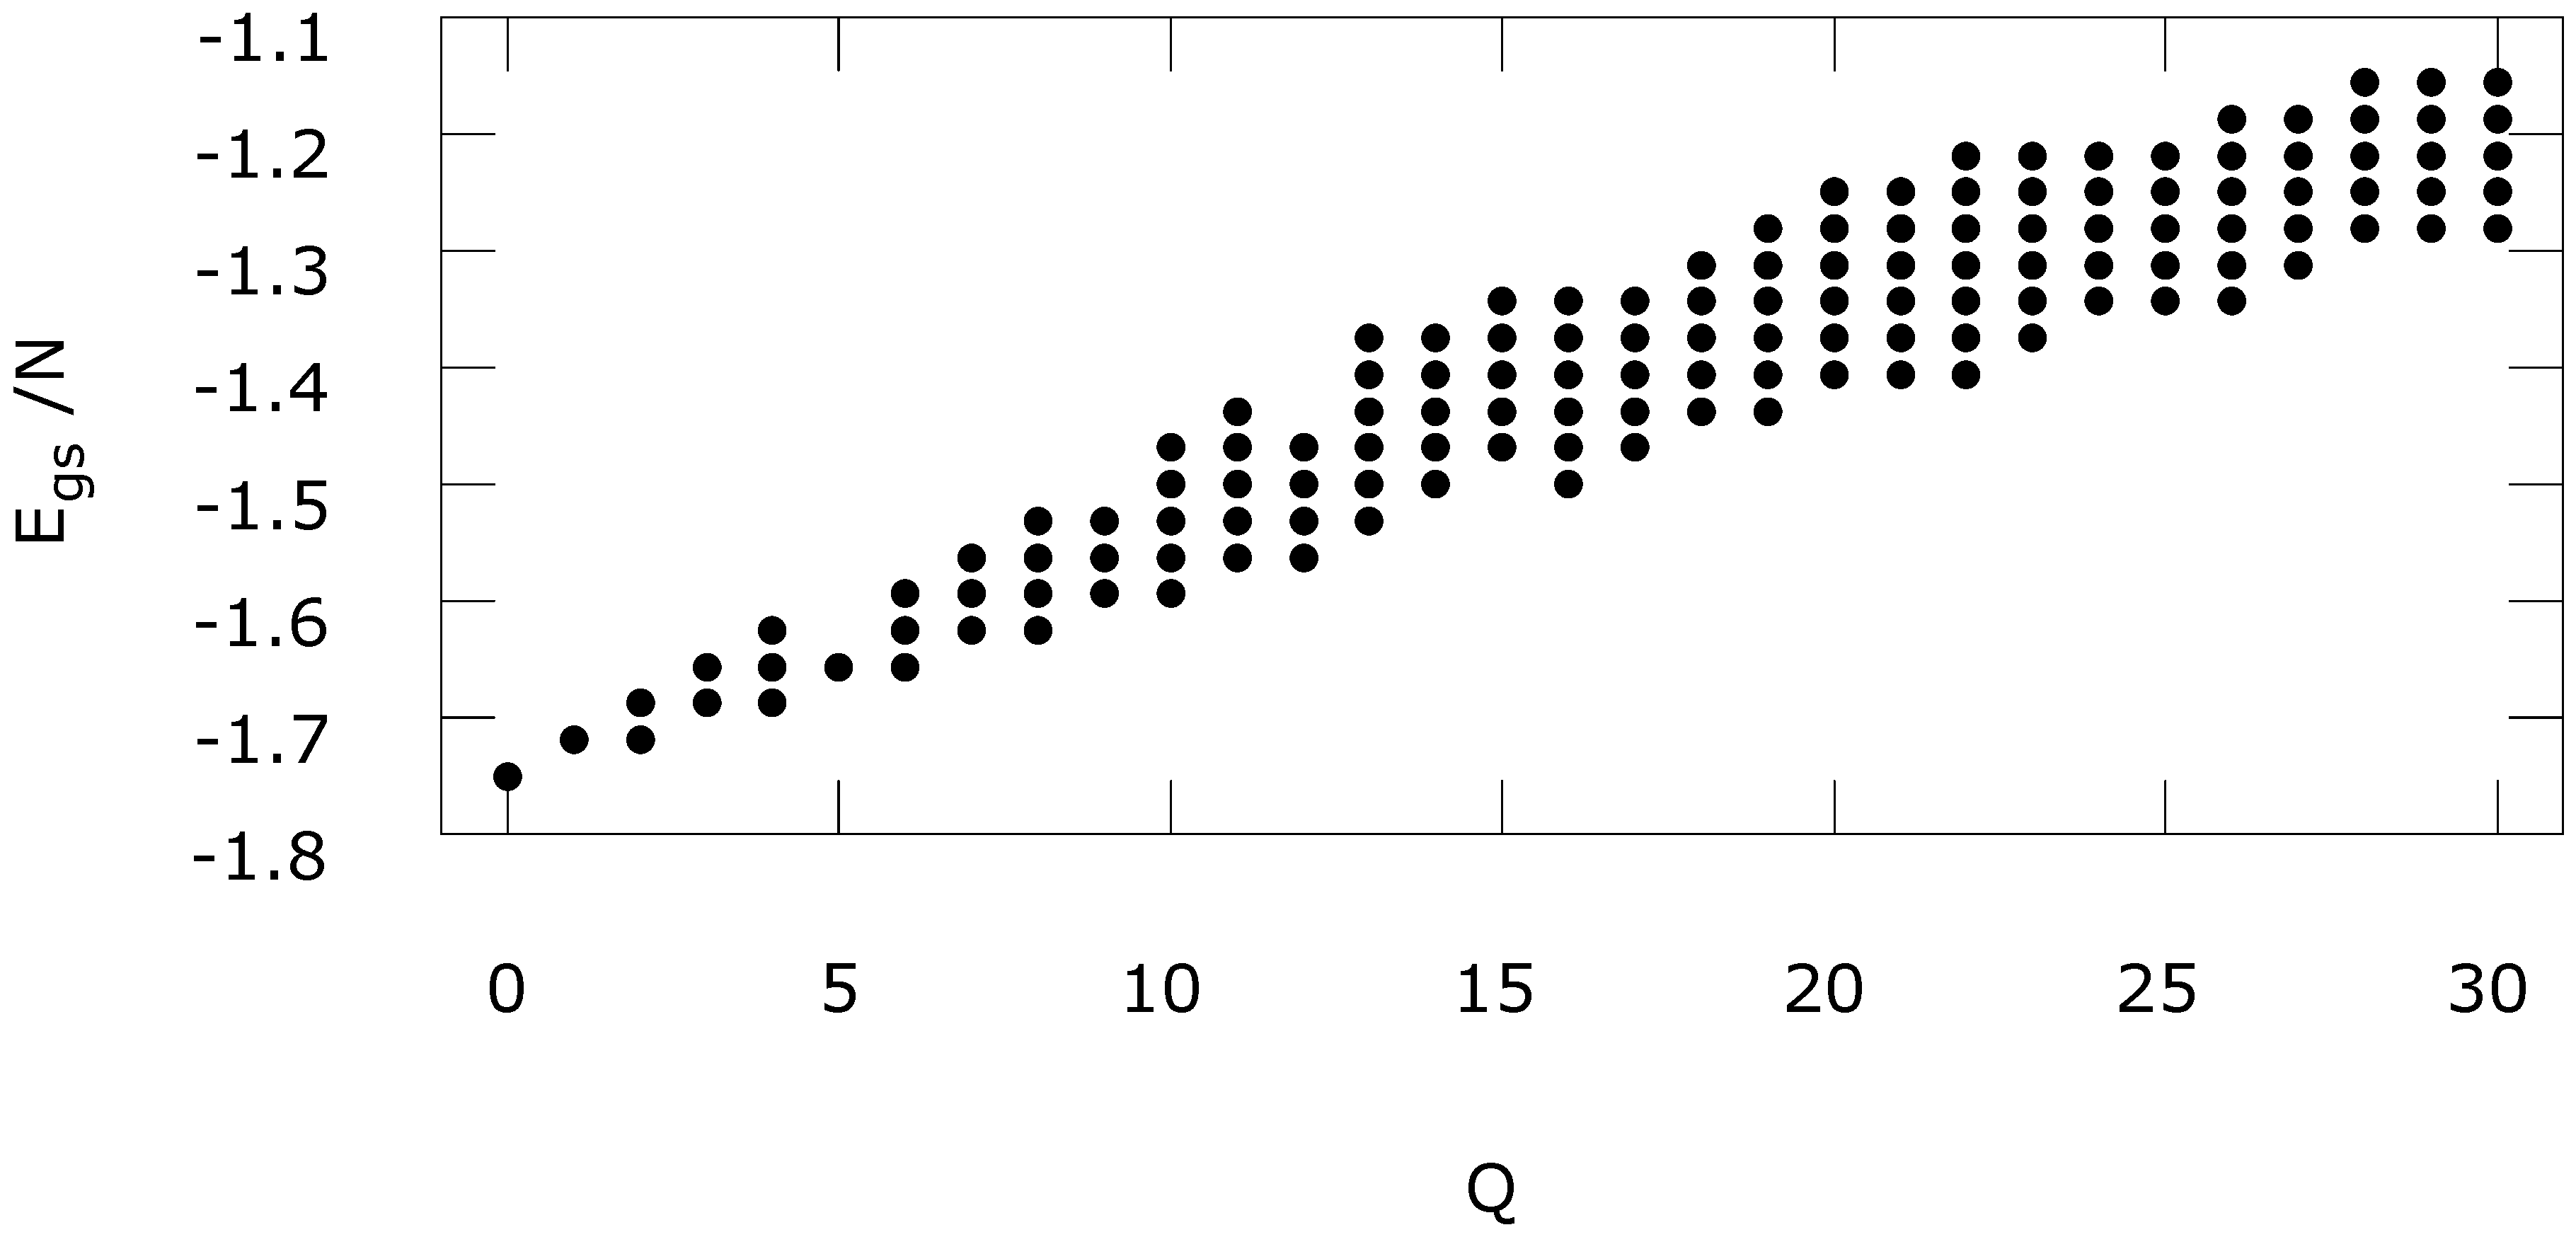
\includegraphics[width=0.5\linewidth]{pictures/E_Q.eps}
	\caption{Ground state energy as a function of the number of Type-II plaquettes for $N=64$}
	\label{fig:E(Q)}
\end{figure}

With an increase in the number of Type-II plaquettes $Q$, the ground state energy increases on average. The rate of energy increase depends not only on the number of Type-II plaquettes but also on their arrangement within the lattice. This explains the variability in ground state energy values shown in Figure \ref{fig:E(Q)} and Table \ref{tab:Egs}.
The increase in ground state energy is driven by the growth in the number of frustrations as the number of Type-II plaquettes increases.


\begin{figure}[H]
	\centering
	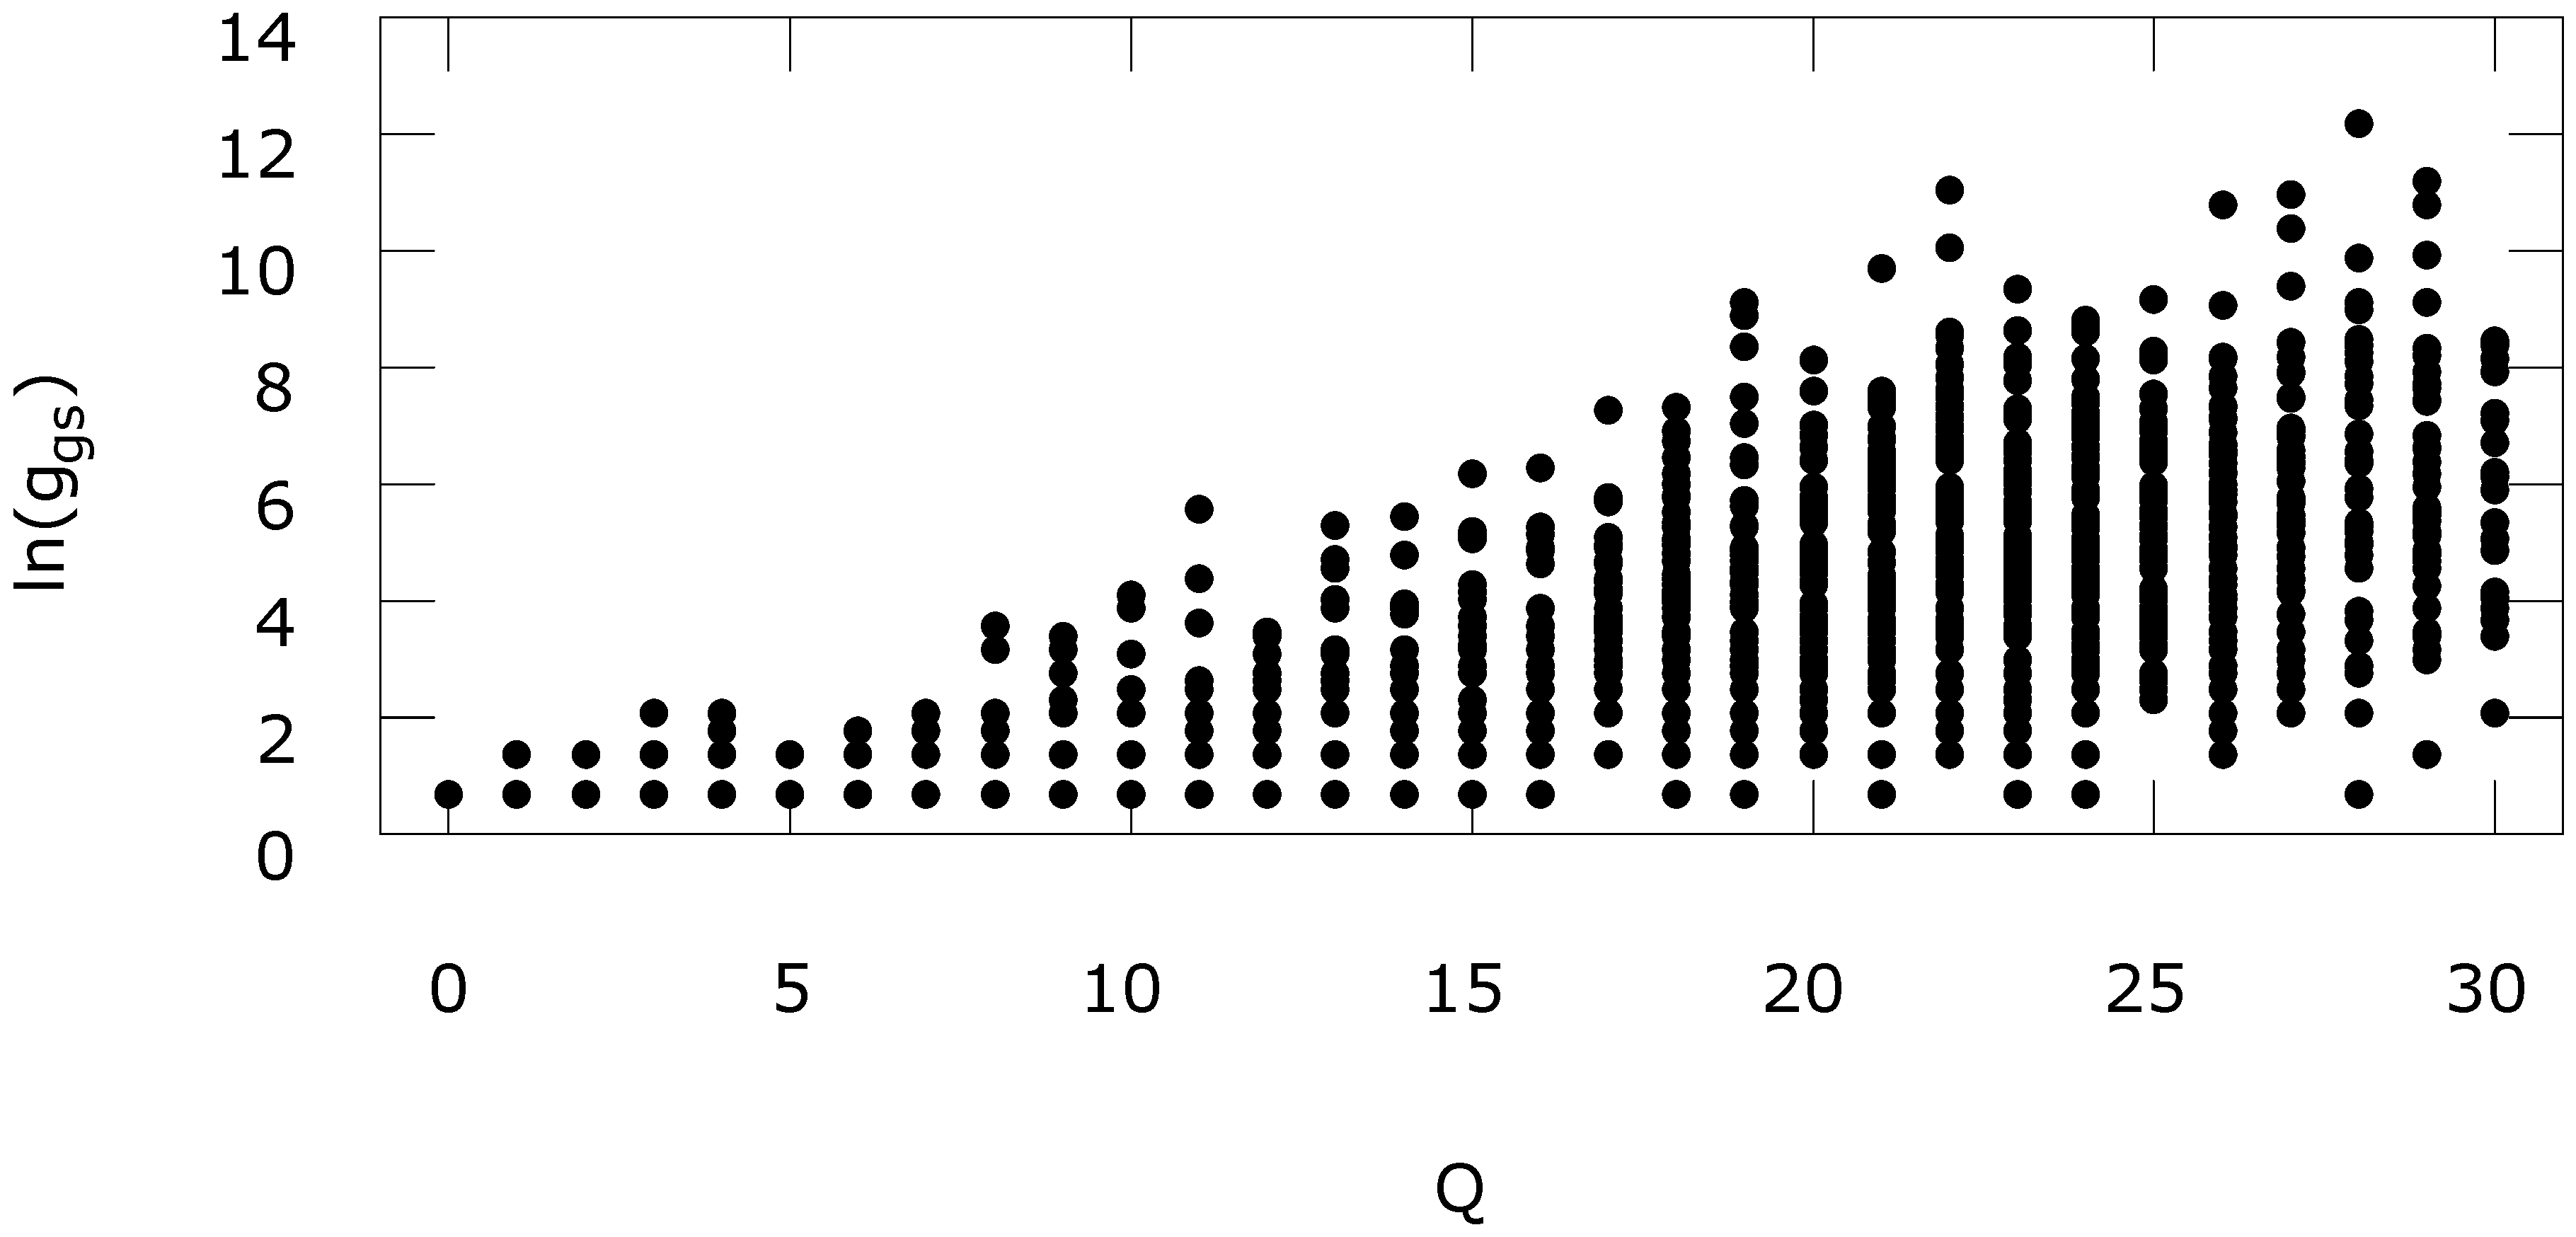
\includegraphics[width=0.5\linewidth]{pictures/g_Q.eps}
	\caption{Ground state degeneracy as a function of the number of Type-II plaquettes for $N=64$}
	\label{fig:g(Q)}
\end{figure}

An increase in the number of Type-II plaquettes, along with the associated rise in the number of frustrations, generally leads to an increase in ground state degeneracy. However, for some samples, an increase in the number of frustrations does not result in a growth in ground state degeneracy (see points with the minimum value $g_{gs}=2$ in Figure \ref{fig:g(Q)}). 

\section{Ground state in an external magnetic field}

Table \ref{tab:Egs} presents the ground state energy values of spin glass. Figure \ref{fig:cell_SI_SG_64} illustrates cases of spin ice and spin glass, which differ in the ordered or disordered distribution of exchange constants. Calculations show that the ground state energy per spin at $P_+ = 0.5$ and in the absence of an external magnetic field for spin ice models is -1.75 and -0.97 (Figures \ref{fig:cell_SI_SG_64}(a) and \ref{fig:cell_SI_SG_64}(c), respectively), while the specific ground state energy of spin glass in the Edwards-Anderson model is -1.28. Spin ice generally refers to a magnet with periodicity in ferromagnetic and antiferromagnetic exchange interactions \cite{peretyatko2017interplay, otsuka2018husimi, andriushchenko2019large, shevchenko2017effect, kato2022flux}. 

\begin{figure}[H]
	\begin{minipage}[h]{0.3\linewidth}
		\centering(a)
		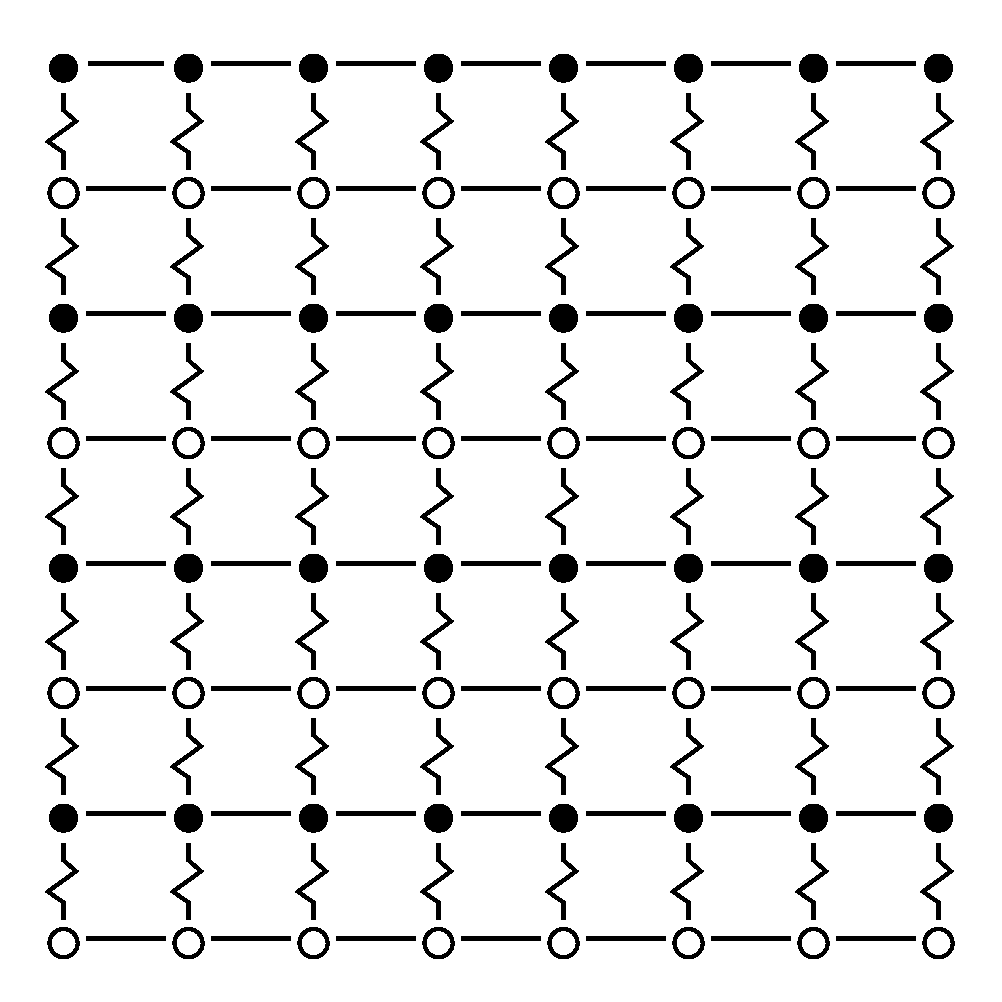
\includegraphics[width=1\linewidth]{pictures/SI_64_J0_1}
	\end{minipage}
	\hfill
	\begin{minipage}[h]{0.3\linewidth}
	\centering(b)
	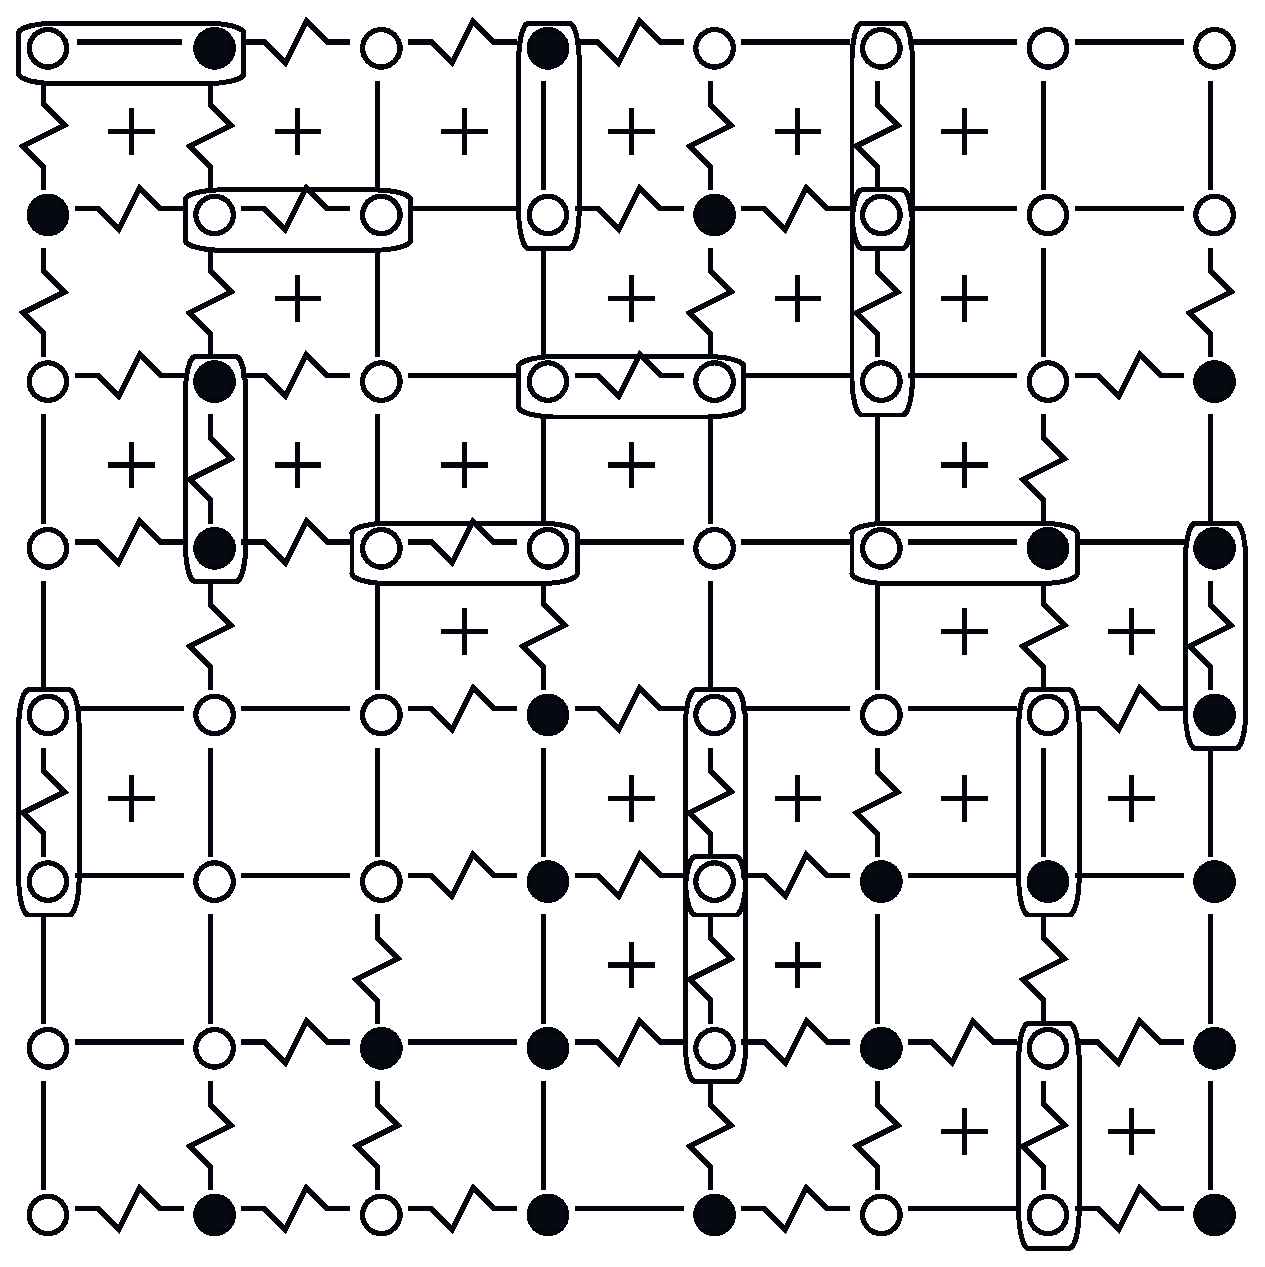
\includegraphics[width=1\linewidth]{pictures/SG_64_J0}
	\end{minipage}
	\hfill
	\begin{minipage}[h]{0.3\linewidth}
		\centering(c)
		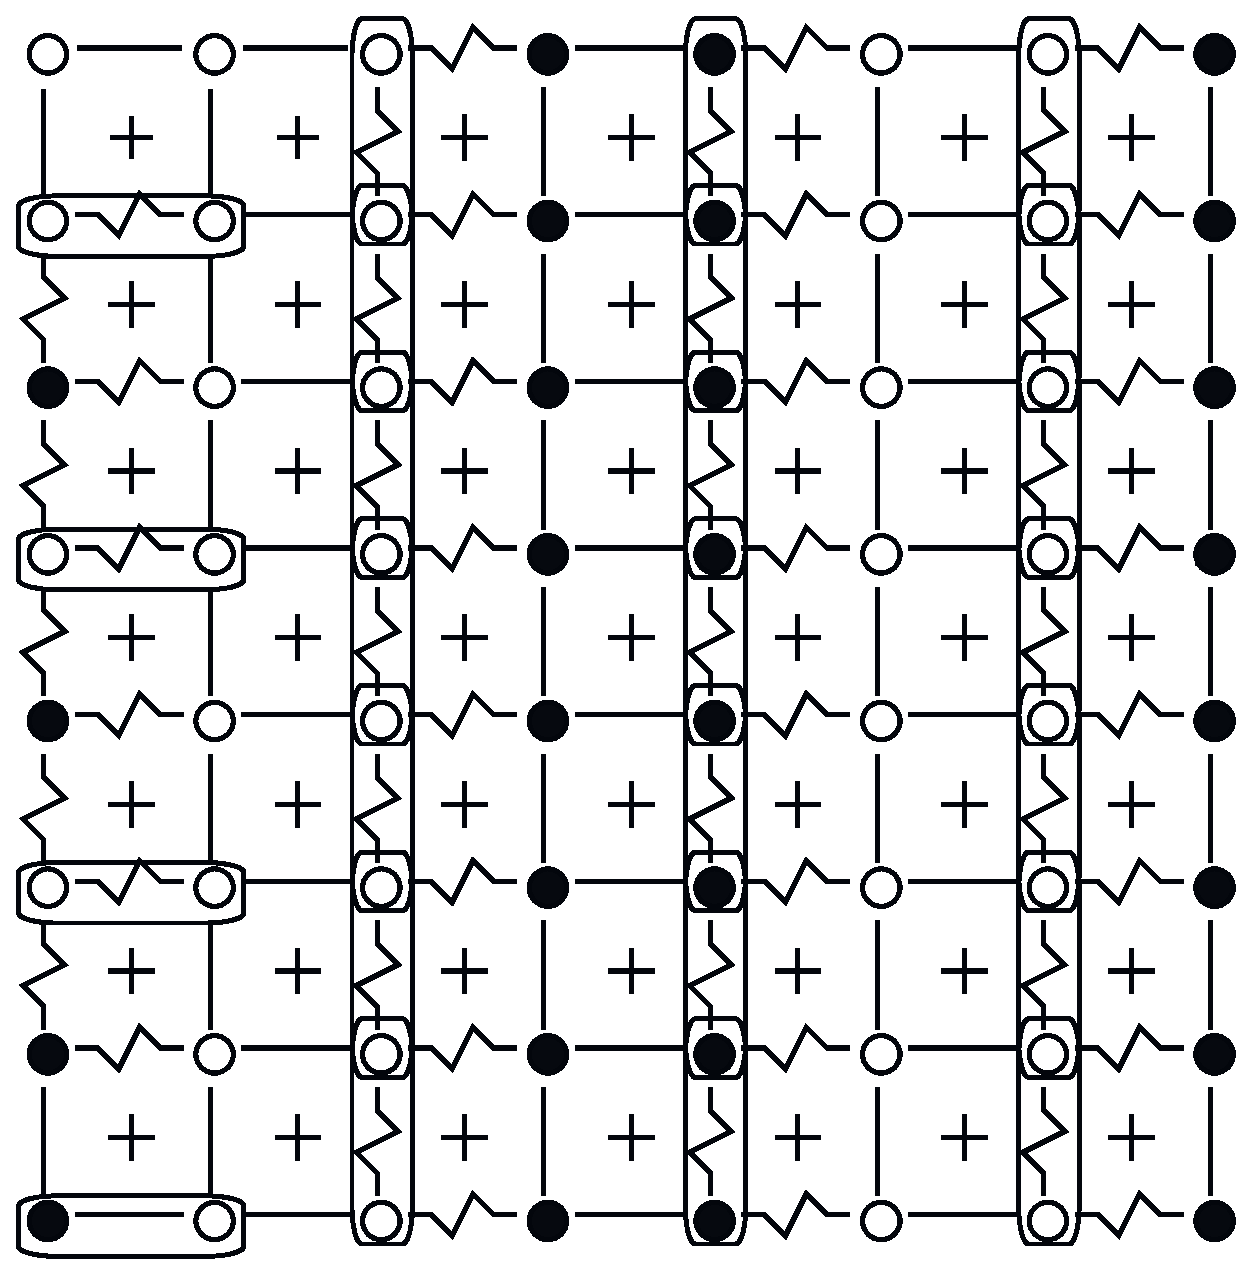
\includegraphics[width=1\linewidth]{pictures/SI_64_J0}
	\end{minipage}
	\hfill
	\caption{Spin ice (a, c) and spin glass (b) lattices consisting of 64 spins with an exchange constant distribution of $P_+ = 0.5$}
	\label{fig:cell_SI_SG_64}

\end{figure}


Figure \ref{fig:cell_SI_SG_64}(a) shows a planar lattice of spin ice composed of Type-I plaquettes, completely free of frustrations.
Figure \ref{fig:cell_SI_SG_64}(b) depicts a spin glass lattice containing 49 plaquettes, of which 16 are of the Type-I, 27 are of Type-II, and 6 are of the Type-III, with a total of 15 frustrations.
In the spin ice lattice shown in Figure \ref{fig:cell_SI_SG_64}(c), the maximum number of frustrations in this example is achieved by filling the system with Type-II plaquettes, resulting in 25 frustrations across 49 plaquettes.


\begin{figure}[H]
	\begin{minipage}[h]{0.32\linewidth}
		\centering(a)
		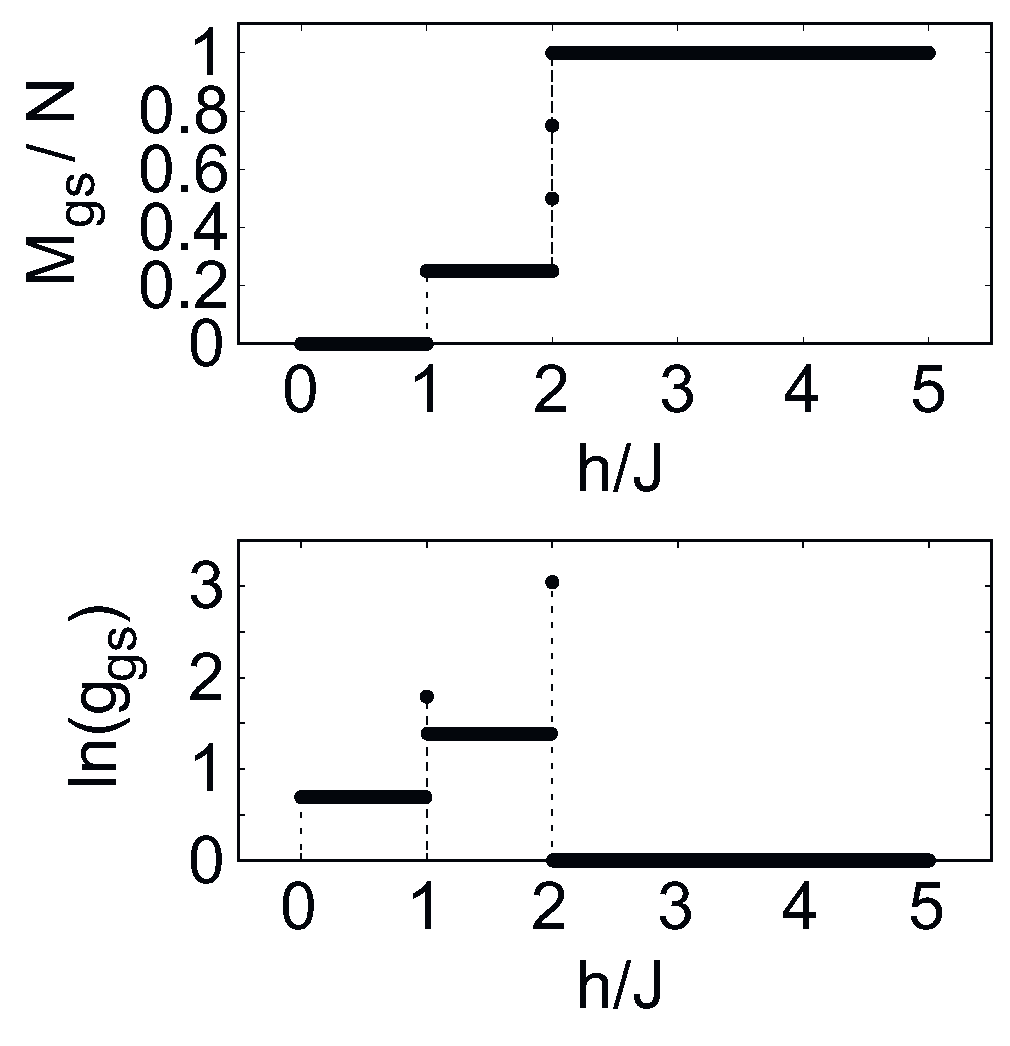
\includegraphics[width=1\linewidth]{pictures/_multiplot_SI64_J0_1}
	\end{minipage}
	\hfill
	\begin{minipage}[h]{0.32\linewidth}
		\centering(b)
		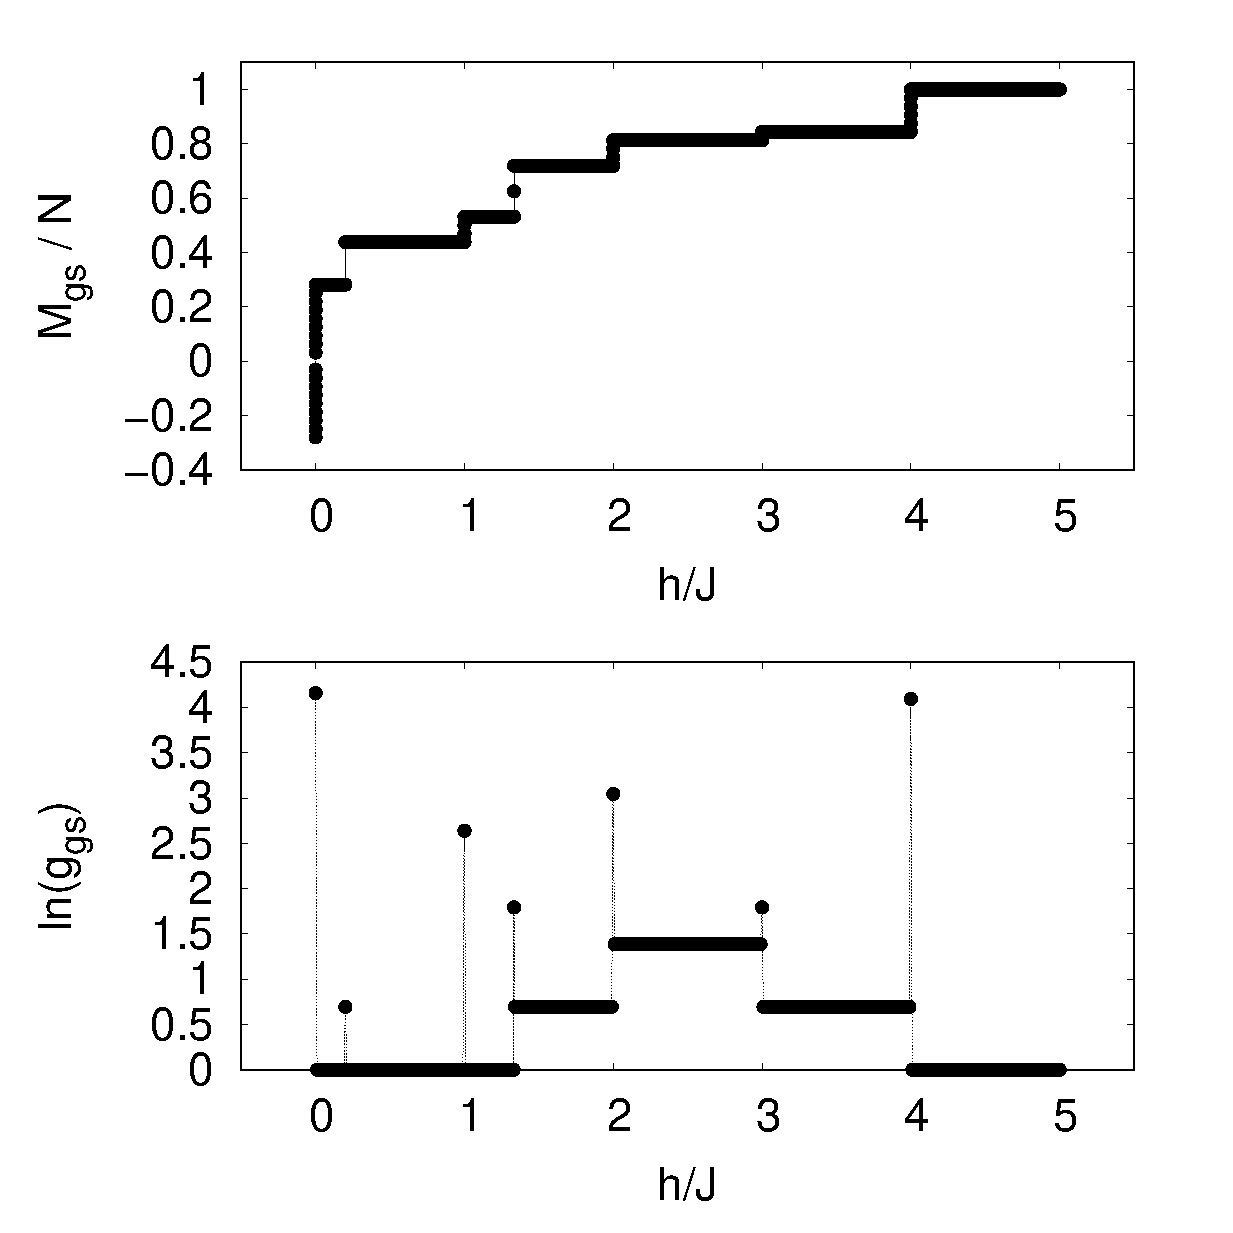
\includegraphics[width=1\linewidth]{pictures/_multiplot_SG64_J0}
	\end{minipage}
	\hfill
	\begin{minipage}[h]{0.32\linewidth}
		\centering(c)
		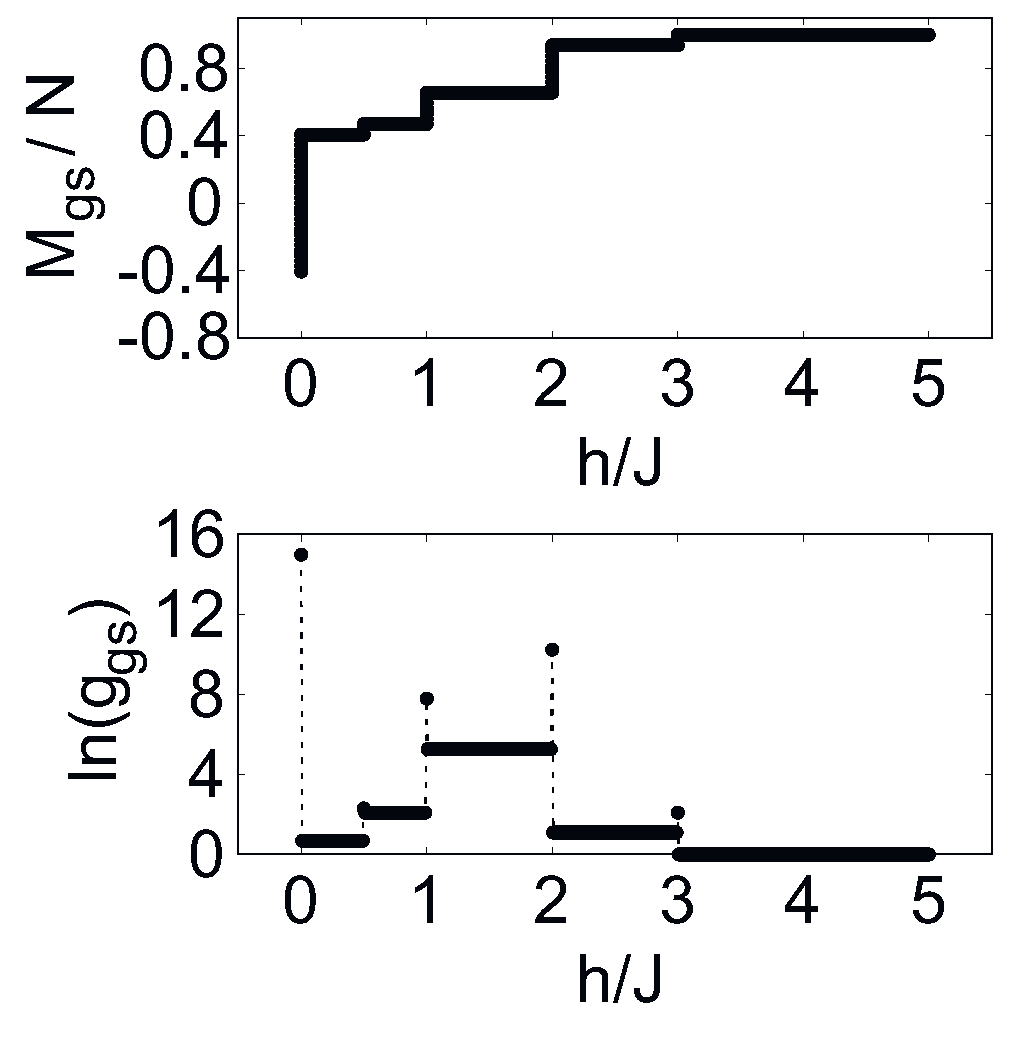
\includegraphics[width=1\linewidth]{pictures/_multiplot_SI64_J0}
	\end{minipage}
	
	\caption{Spin excess and residual entropy of spin ice (a, c) and spin glass (b) (exchange constant distribution shown in Figure \ref{fig:cell_SI_SG_64})}
	\label{fig:_multiplot_SI_SG_64}
	
\end{figure}


Figure \ref{fig:_multiplot_SI_SG_64} shows the dependencies of spin excess and ground state degeneracy on the external magnetic field strength.
In the absence of frustrations and an external magnetic field, the ground state of spin ice is doubly degenerate (Figure \ref{fig:_multiplot_SI_SG_64}(a)).
In spin glass, the introduction of frustrations increases the ground state degeneracy to 64 (Figure \ref{fig:_multiplot_SI_SG_64}(b)).
Maximal filling of the spin ice system with frustrated Type-II plaquettes leads to macroscopic ground state degeneracy, with the number of degenerate configurations exceeding $3\times10^{6}$ (Figure \ref{fig:_multiplot_SI_SG_64}(c)).



Under the influence of an external magnetic field, the spin glass system exhibits the highest number of steps in the spin excess graph (Figure \ref{fig:_multiplot_SI_SG_64}(b)).
This number is determined not by the number of frustrations but by the shape of the density of states (DOS), which plays a significant role.
It is worth noting that the number of steps implicitly depends on the number of frustrations.

Using complete enumeration method, the densities of states were constructed for the spin ice and spin glass samples shown in Figure \ref{fig:cell_SI_SG_64}, as functions of external magnetic field strength (Figures \ref{fig:HDOS_ice_1}, \ref{fig:HDOS_glass}, and \ref{fig:HDOS_ice}).
The system's energy under the influence of an external magnetic field was calculated using Equation (\ref{eq:ising_energy}).

\begin{figure}[H]
	\centering
	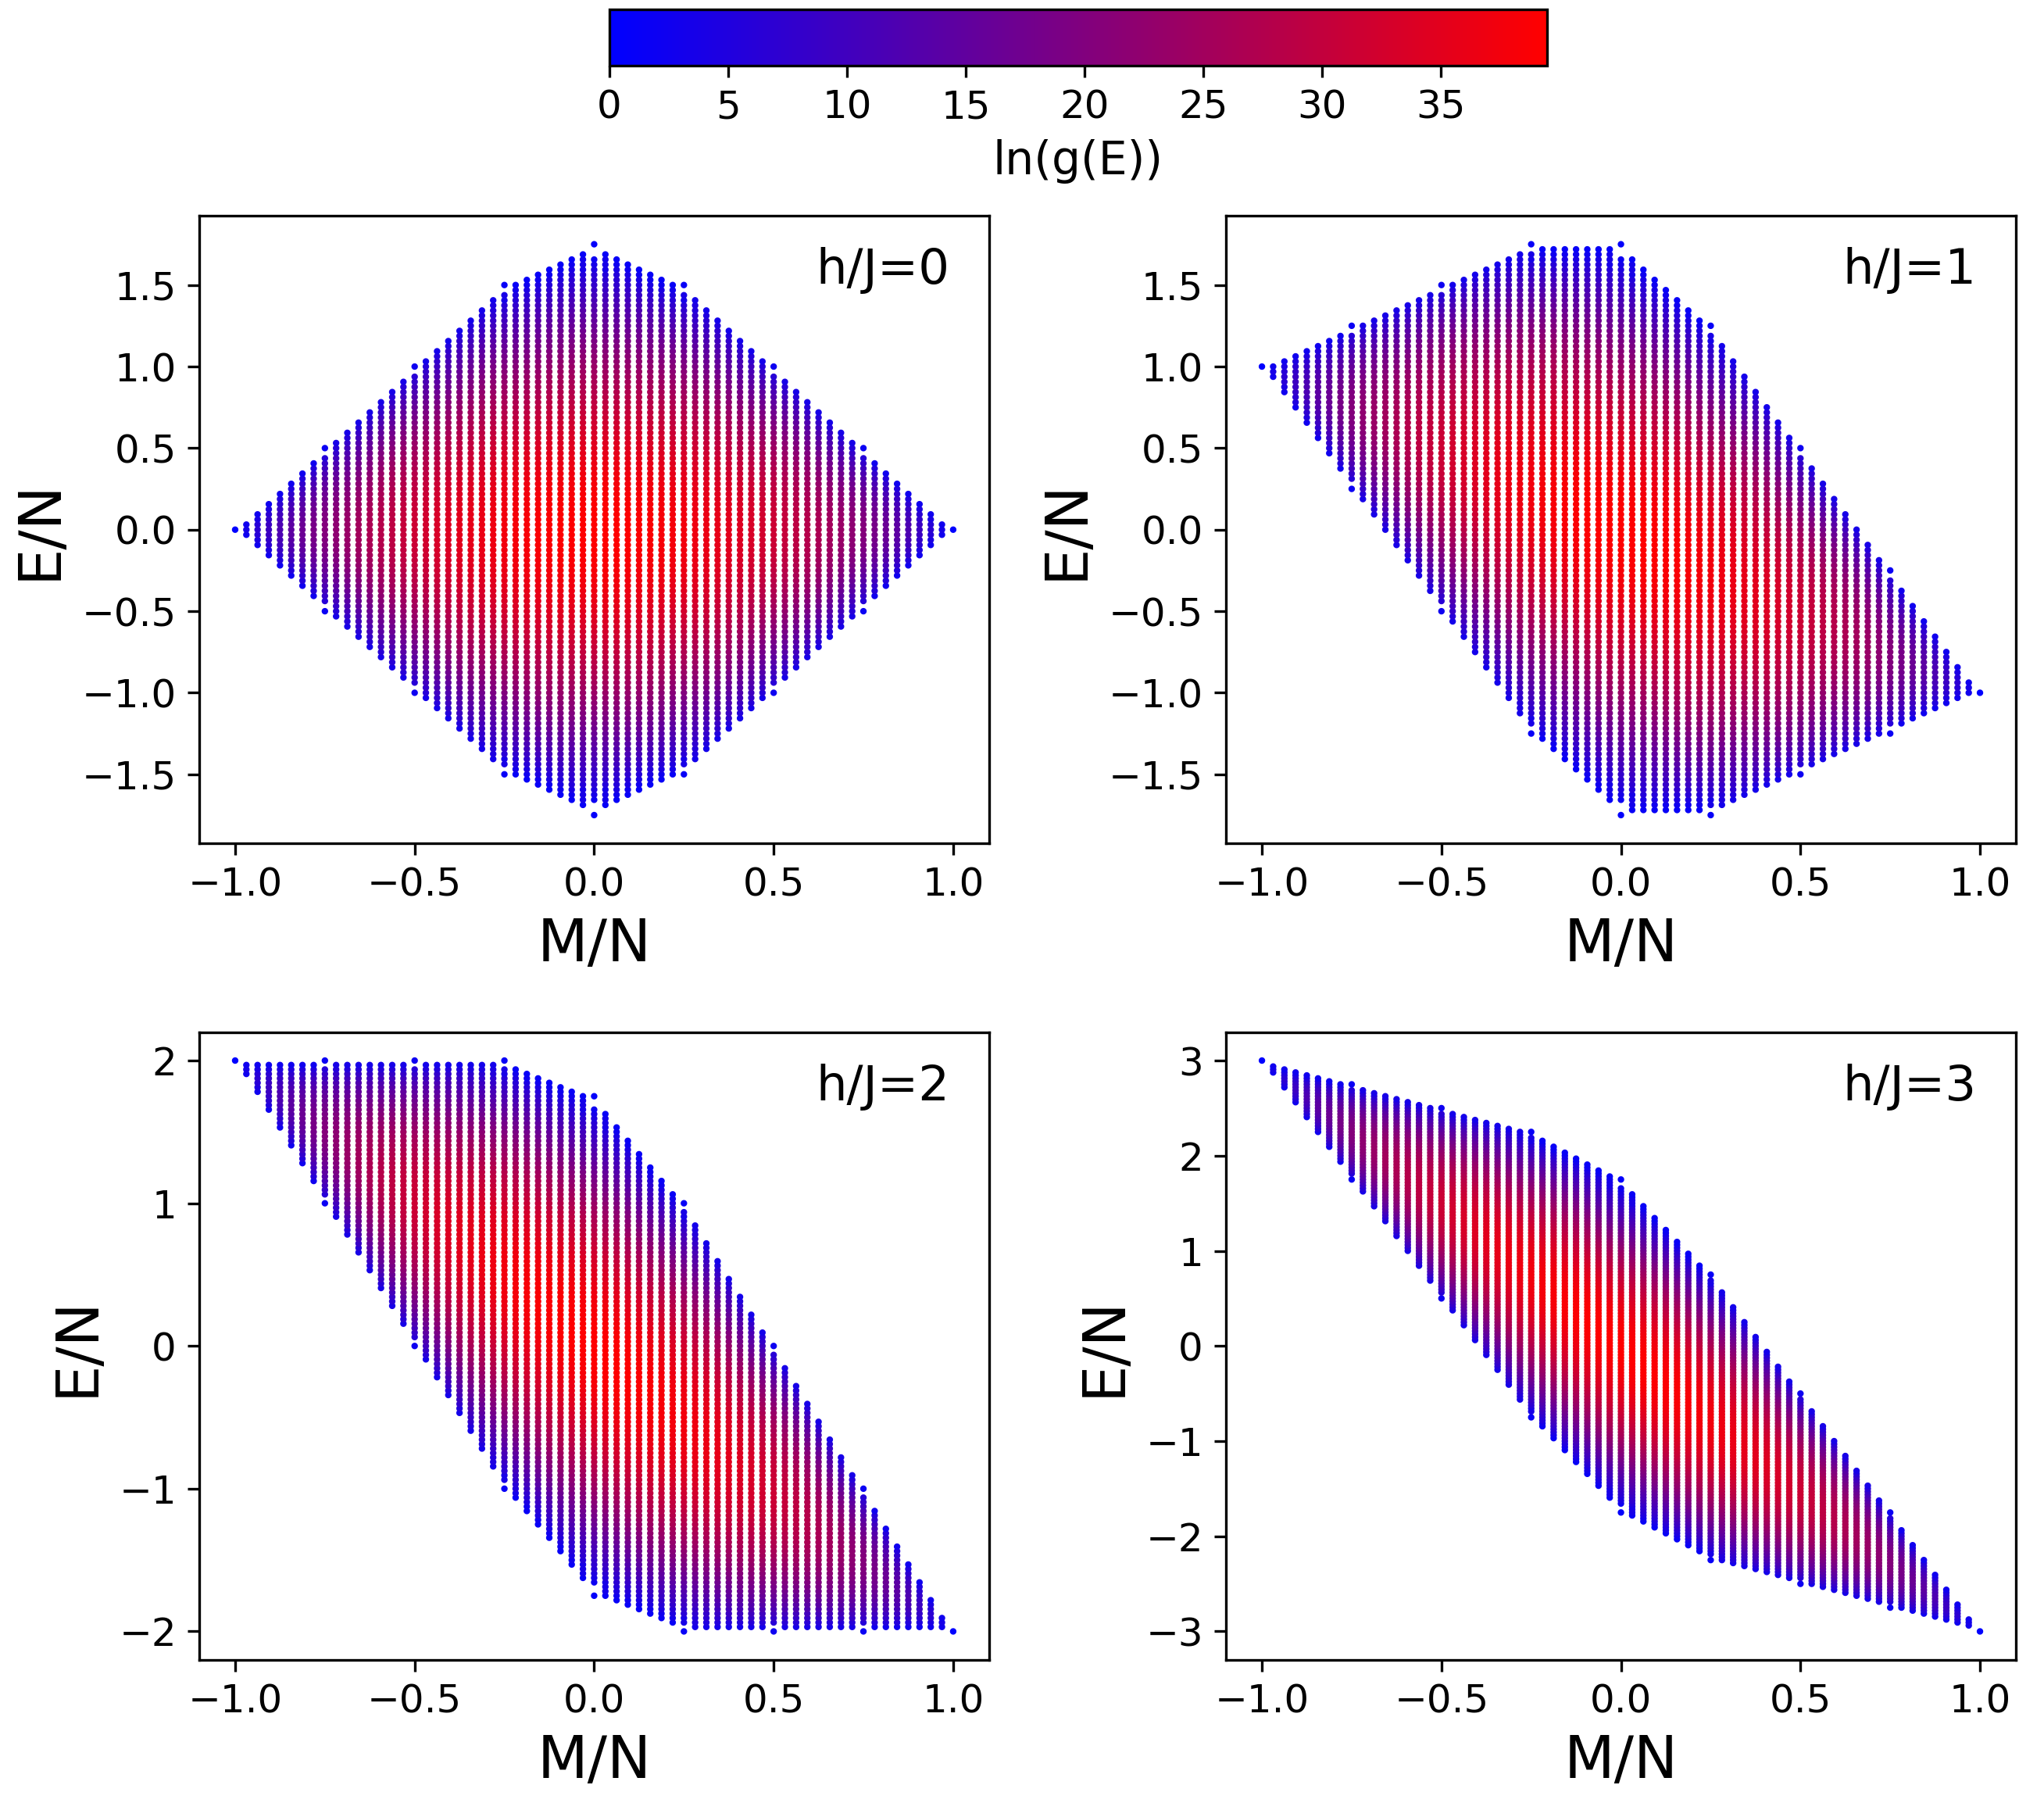
\includegraphics[width=1\linewidth]{pictures/HDOS_SI_64_J0_1.png}
	\caption{Density of states in an external magnetic field $0\leq h/J \leq 2$ for the spin ice lattice (exchange constant distribution shown in Figure \ref{fig:cell_SI_SG_64}(a))}
	\label{fig:HDOS_ice_1}
\end{figure}

\begin{figure}[H]
		\centering
		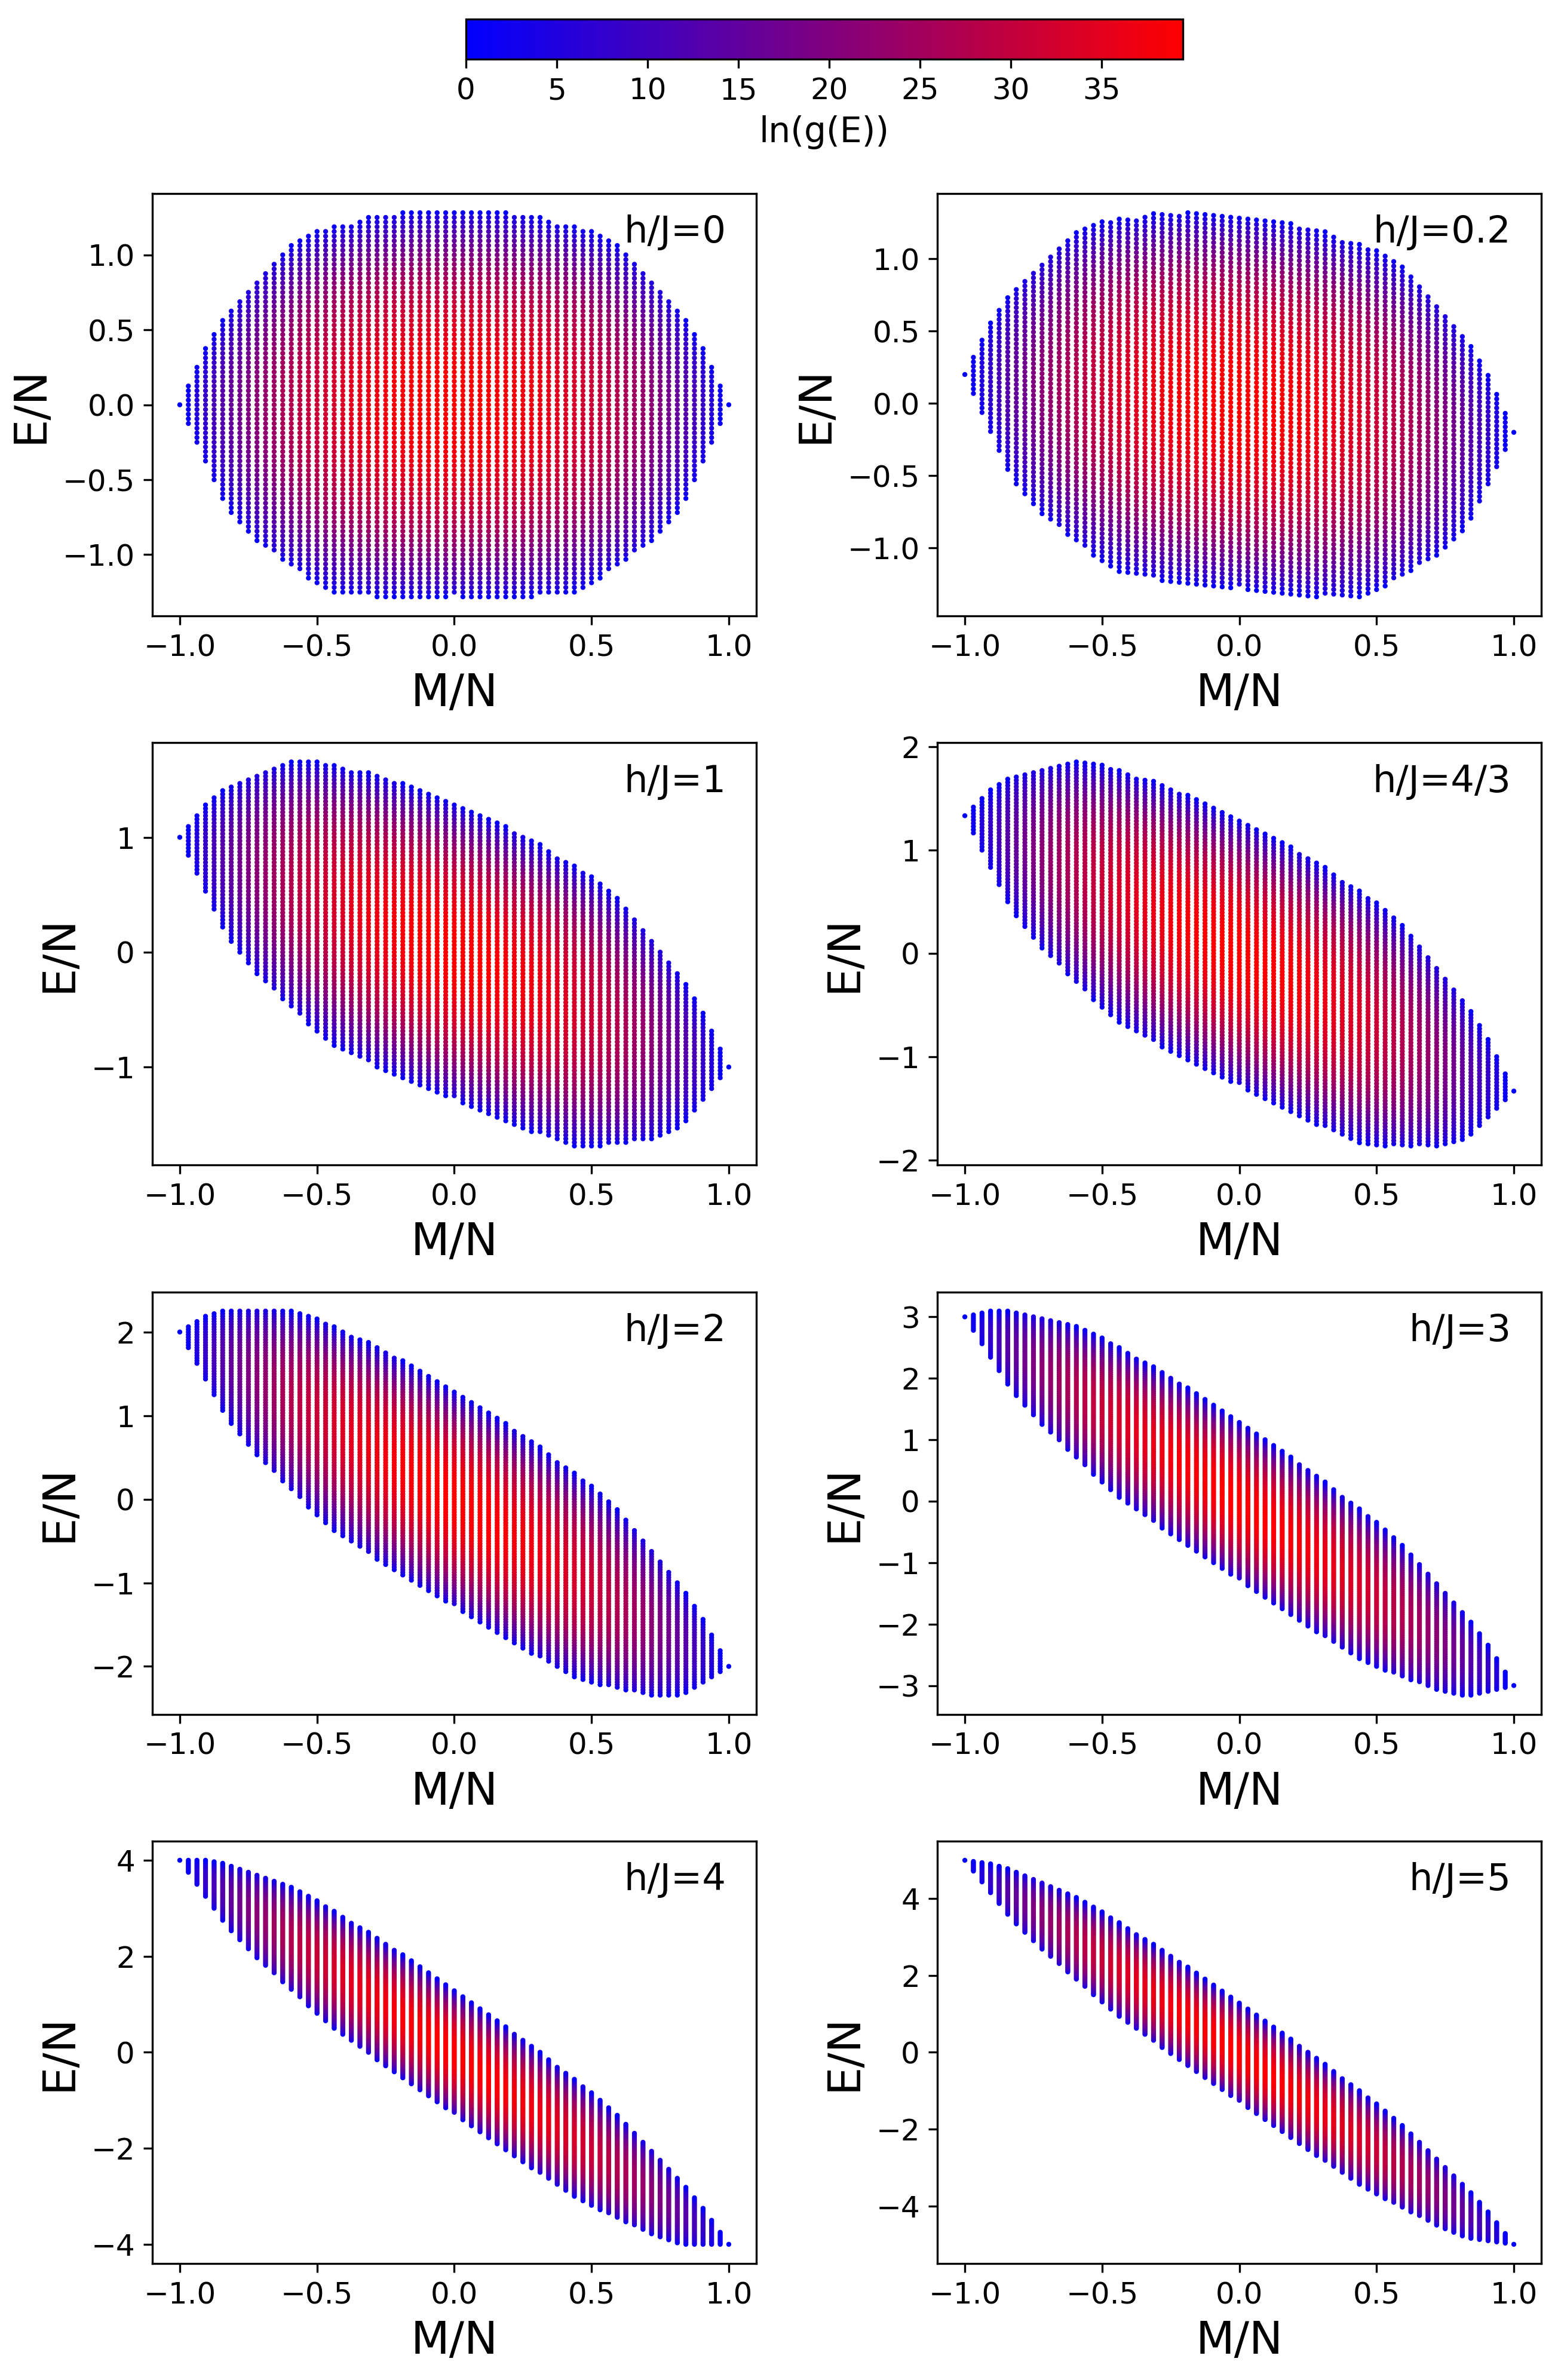
\includegraphics[width=1\linewidth]{pictures/HDOS_SG_64_J0.png}
	\caption{Density of states in an external magnetic field $0\leq h/J \leq 5$ for the spin glass lattice (exchange constant distribution shown in Figure \ref{fig:cell_SI_SG_64}(b))}
	\label{fig:HDOS_glass}
\end{figure}


\begin{figure}[H]
	\centering
	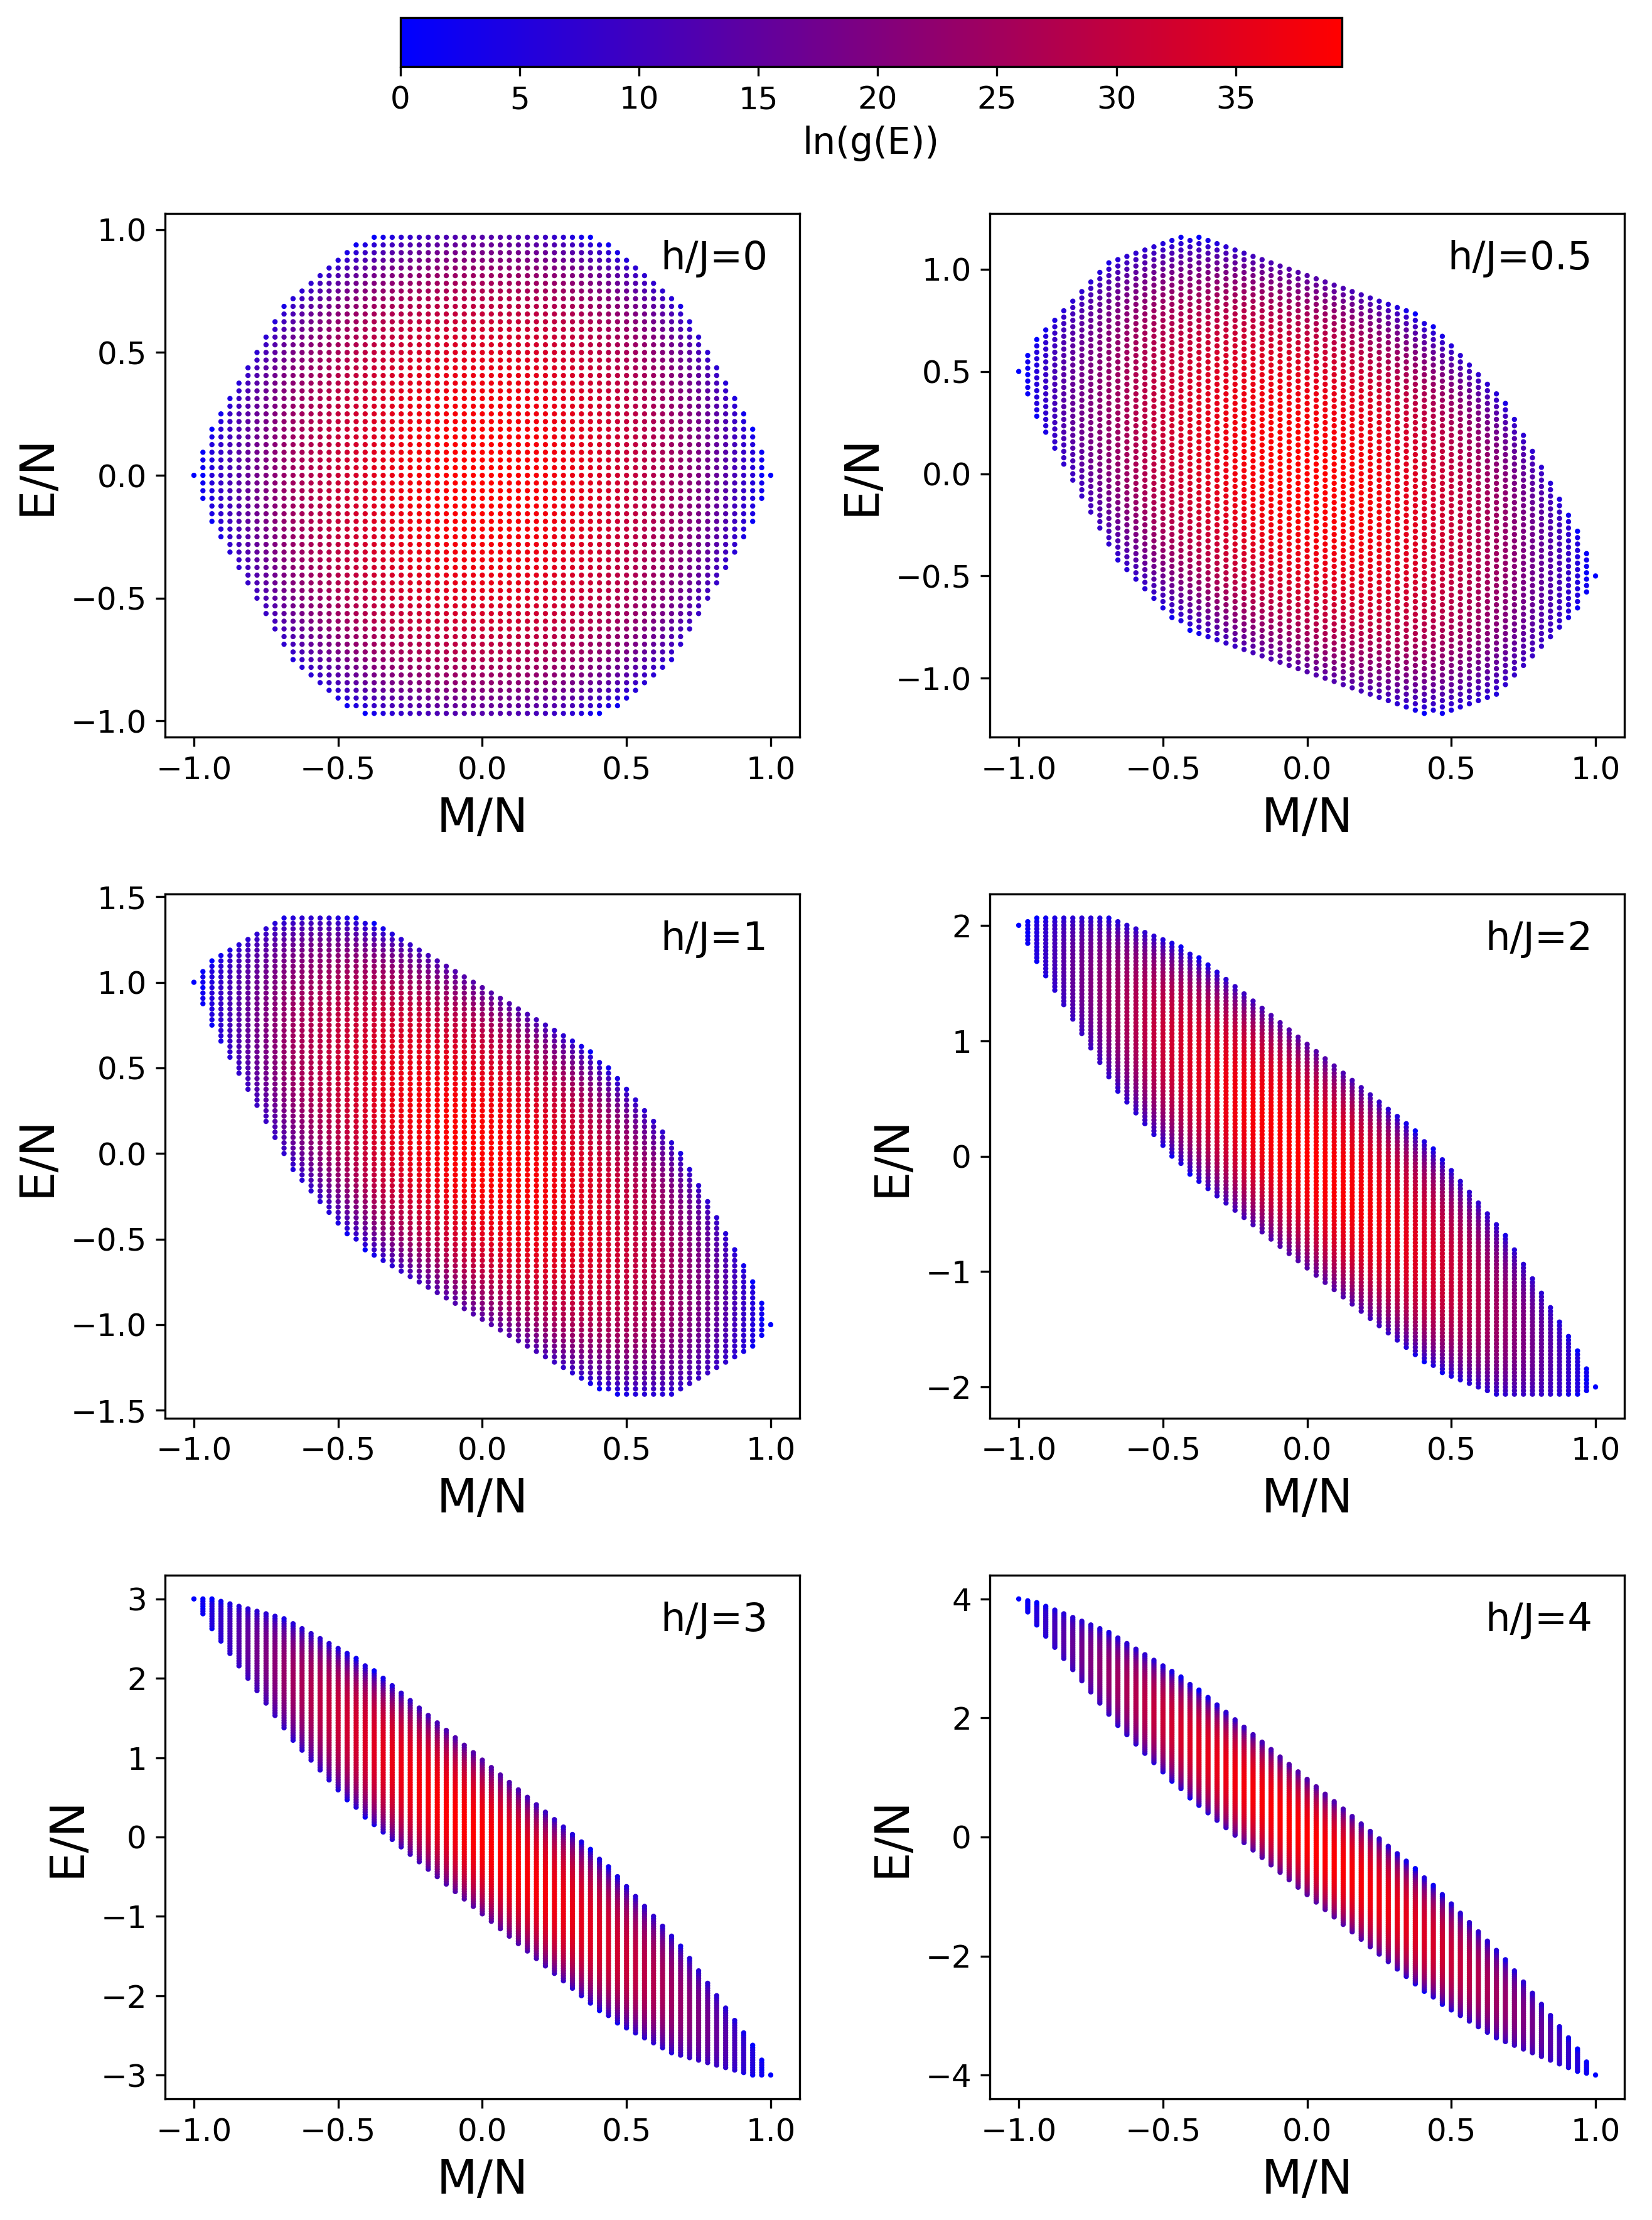
\includegraphics[width=1\linewidth]{pictures/HDOS_SI_64_J0.png}
	\caption{Density of states in an external magnetic field $0\leq h/J \leq 4$ for the spin ice lattice (exchange constant distribution shown in Figure \ref{fig:cell_SI_SG_64}(c))}
	\label{fig:HDOS_ice}
\end{figure}

In Figure \ref{fig:HDOS_ice_1}, at $h/J=0$ for spin ice (Figure \ref{fig:cell_SI_SG_64}(a)), the ground state degeneracy can be observed. An increase in the external magnetic field to the critical value $h/J=1$, due to the growth of the Zeeman energy, results in the ground state energy with spin excess $M=0$ becoming equal to the ground state energy with spin excess $M=0.25$. The entropies of the ground states are summed.
Further increasing the external magnetic field to $h/J=2$ leads to a situation where the ground states correspond to spin excess values of $M=\pm0.25; \pm0.5; \pm0.75; \pm1$.
The value  $h/J=3$ is the saturation field, at which only one configuration remains.


For spin glass (Figure \ref{fig:cell_SI_SG_64}(b)), entropy jumps at $T=0$ in the critical fields are determined by the boundaries of the density of states (see Figure \ref{fig:HDOS_glass}).


Spin ice (Figure \ref{fig:cell_SI_SG_64}(c)) exhibits less variety in critical fields compared to spin glass (see Figure \ref{fig:HDOS_ice}). However, the ground state degeneracy is greater than that of spin glass.


\section{Antiferromagnetism, spin glass, and ferromagnetism at $T = 0$}

The phase diagram at non-zero temperatures in an external magnetic field was studied in \cite{trukhin2024thermodynamic}. Of particular interest is the separation of antiferromagnetic, spin glass, and ferromagnetic phases at $T = 0$).

Table \ref{tab:lit_phase} summarizes theoretical and numerical results for the critical transition point (relative concentration of ferromagnetic bonds $P_+$) from the antiferromagnetic phase to the spin glass phase.

\begin{table}[!h]
	\centering
	\begin{tabular}{|l|c|l|}
		\hline
		Method & \( P_{+} \) & Reference \\ \hline
		Series expansion & ~0.099 & \cite{PhysRevB.19.260} \\ \hline
		Matching algorithm & \( 0.105 \pm 0.01 \) & \cite{H_Freund_1989} \\ \hline
		Matching algorithm & \( 0.095 < p_c < 0.108 \) & \cite{BENDISCH1994139} \\ \hline
		Exact ground states & \( 0.106 \pm 0.002 \) & \cite{N.Kawashima_1997} \\ \hline
		Ground state enumeration & 0.115 & \cite{PhysRevE.58.1502} \\ \hline
		Exact ground states & \( 0.1031 \pm 0.0001 \) & \cite{WANG200331} \\ \hline
		Exact ground states & \( 0.103 \pm 0.001 \) & \cite{amoruso2004domain} \\ \hline
	\end{tabular}
	\caption{Critical point for the AFM-SG transition (ferromagnetic bond concentration \( P_+ \))}
	\label{tab:lit_phase}
\end{table}

Figure \ref{fig:Mgs(P+)} shows the dependence of the maximum spin excess in the ground state on the relative number of ferromagnetic bonds $P_+$. The density of ferromagnetic bonds is determined by $P_+$, and bonds are randomly distributed while maintaining $P_+$ within each series. Each series consisted of 10 samples for numerical calculations.

\begin{figure}[H]
	\centering
	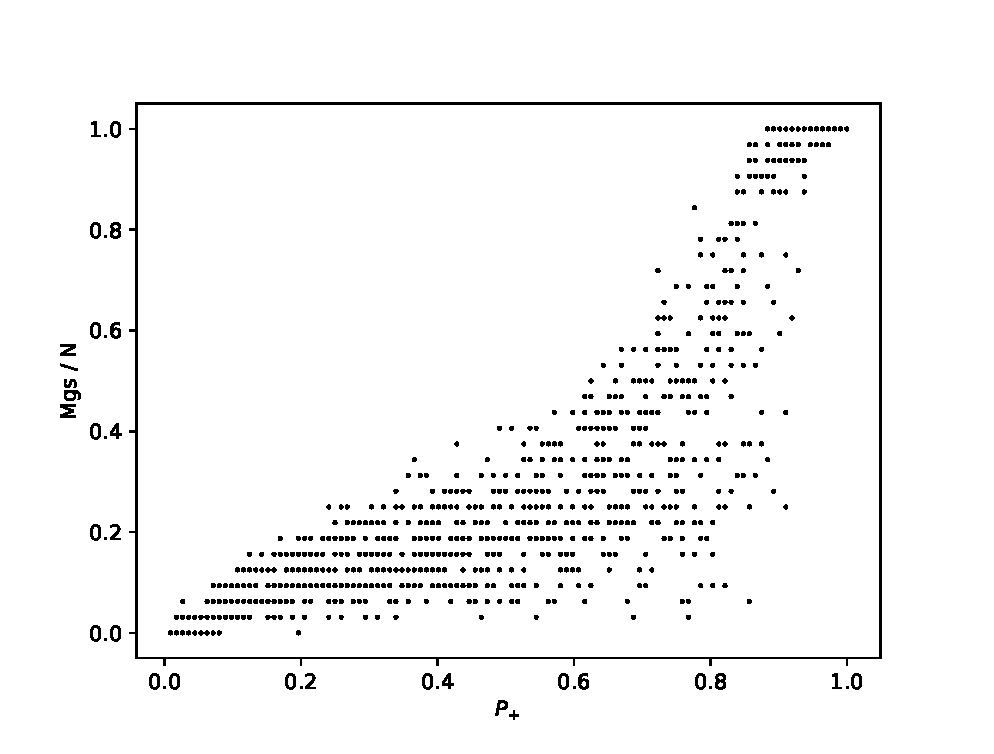
\includegraphics[width=0.8\textwidth]{images/Mgs(P+).eps}
	\caption{Maximum ground state spin excess as a function of the relative number of ferromagnetic bonds $P_+$}
	\label{fig:Mgs(P+)}
\end{figure}

For a pure ferromagnet ($P_+ = 1.0$), the spin excess equals the number of spins ($M/N = 1.0$), while for a pure antiferromagnet, it is zero (in the case of an even number of spins). For a given $P_+$, the ratio of points where the maximum ground state spin excess equals zero to the number of points where $M_{gs}/N \neq 0.0$ represents the probability of an antiferromagnetic state, as shown in Figure \ref{fig:P_AFM_FM_Mmax}(a). Similarly, the ratio of points with $M_{gs}/N = 1.0$ (ferromagnetic spin excess) to the number of points where $M_{gs}/N \neq 1.0$ represents the probability of a ferromagnetic state, as shown in Figure \ref{fig:P_AFM_FM_Mmax}(b).

\begin{figure}[H]
	\begin{minipage}[h]{0.45\linewidth}
		\centering (a)
		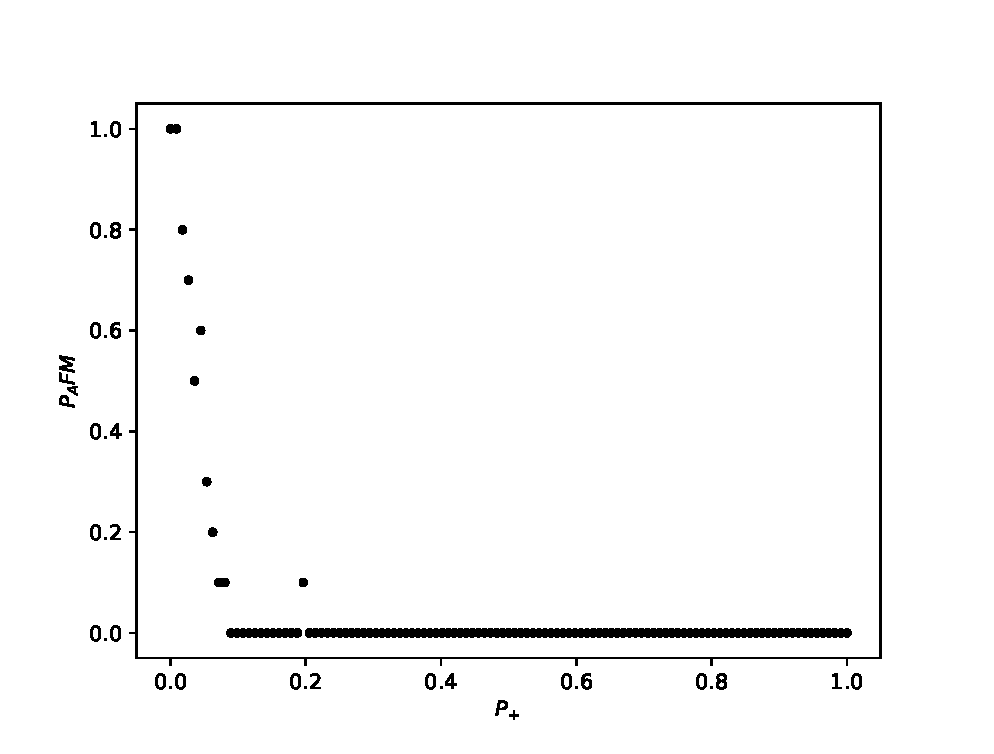
\includegraphics[width=1\linewidth]{images/P_AFM_Mmax.eps}
	\end{minipage}
	\hfill
	\begin{minipage}[h]{0.45\linewidth}
		\centering (b)
		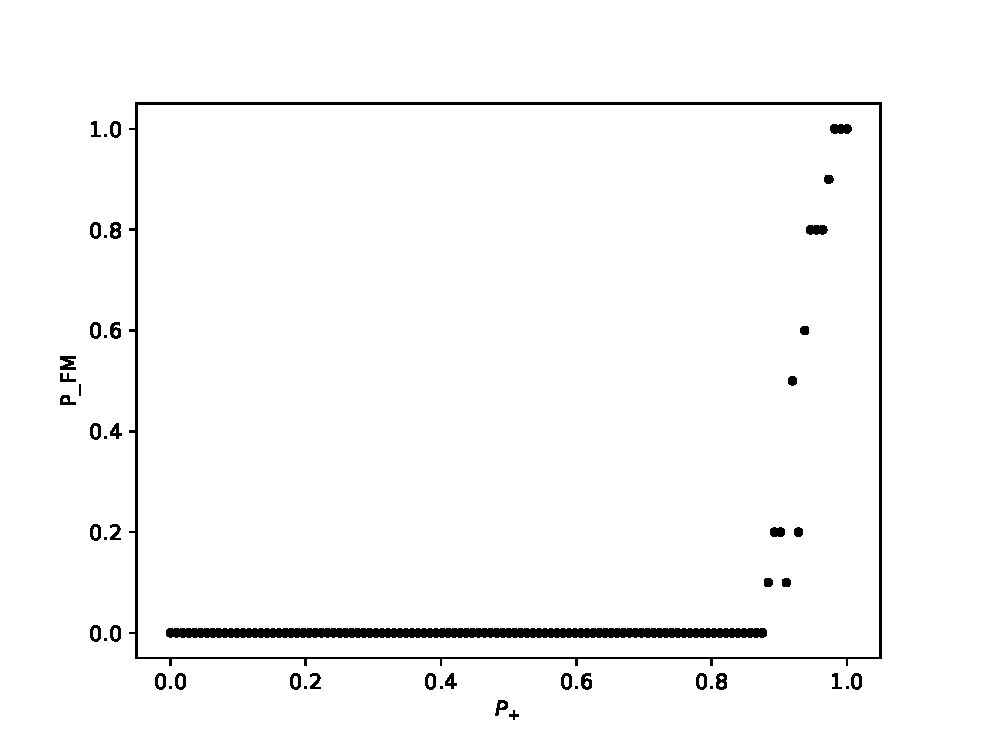
\includegraphics[width=1\linewidth]{images/P_FM_Mmax.eps}
	\end{minipage}
	\caption{Probability of antiferromagnetic (a) and ferromagnetic (b) states at \( T = 0 \)}
	\label{fig:P_AFM_FM_Mmax}
\end{figure}

The antiferromagnetic phase at $T = 0$ occurs for $0.0 \leq P_+ \leq 0.1$. The spin glass phase is realized for $0.1 \leq P_+ \leq 0.9$. The ferromagnetic phase occurs for $0.9 \leq P_+ \leq 1.0$. These results align with the critical values for the antiferromagnetic phase in Table \ref{tab:lit_phase} and provide boundaries for the ferromagnetic phase at zero temperature in the absence of an external magnetic field.

The complete density of states allows reliable calculation of sample properties in an external magnetic field. Under an external magnetic field ($h/J = 1$ and $h/J = 2$), the proportion of the ferromagnetic phase increases while that of the antiferromagnetic phase decreases, as shown in Figure \ref{fig:Mgs(P+)_H}. Phase transition points under an external field exhibit behavior similar to \cite{trukhin2024thermodynamic}.

\begin{figure}[H]
	\begin{minipage}[h]{0.45\linewidth}
		\centering (a)
		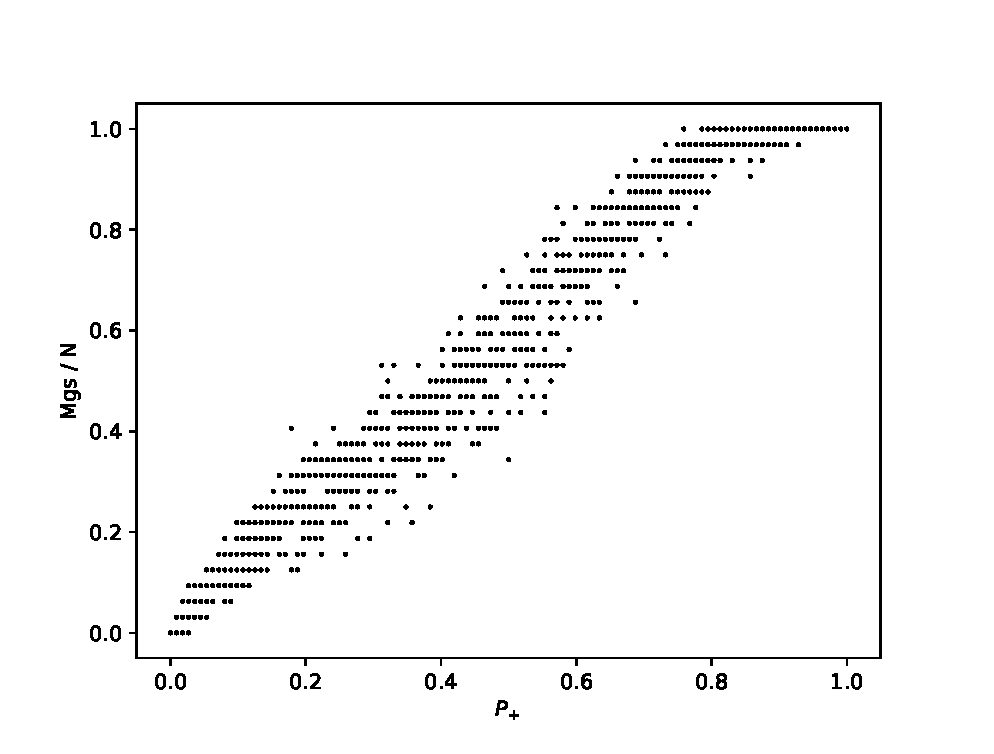
\includegraphics[width=1\linewidth]{images/Mgs(P+)_H1.eps}
	\end{minipage}
	\hfill
	\begin{minipage}[h]{0.45\linewidth}
		\centering (b)
		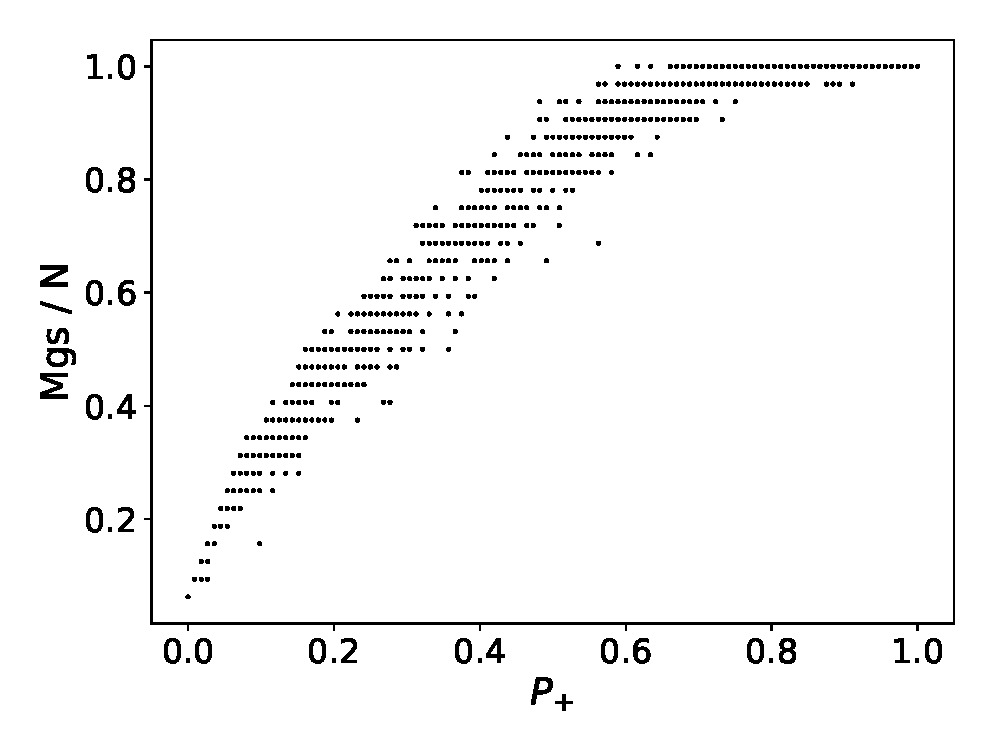
\includegraphics[width=1\linewidth]{images/Mgs(P+)_H2.eps}
	\end{minipage}
	\caption{Ground state spin excess for all values of bond distribution density under external fields $h/J = 1$ (a) and $h/J = 2$ (b)}
	\label{fig:Mgs(P+)_H}
\end{figure}

The theoretical ground state phase diagram ($h-P_+$) is shown in Figure \ref{fig:P+_afm_fm(H)}.

\begin{figure}[H]
	\centering
	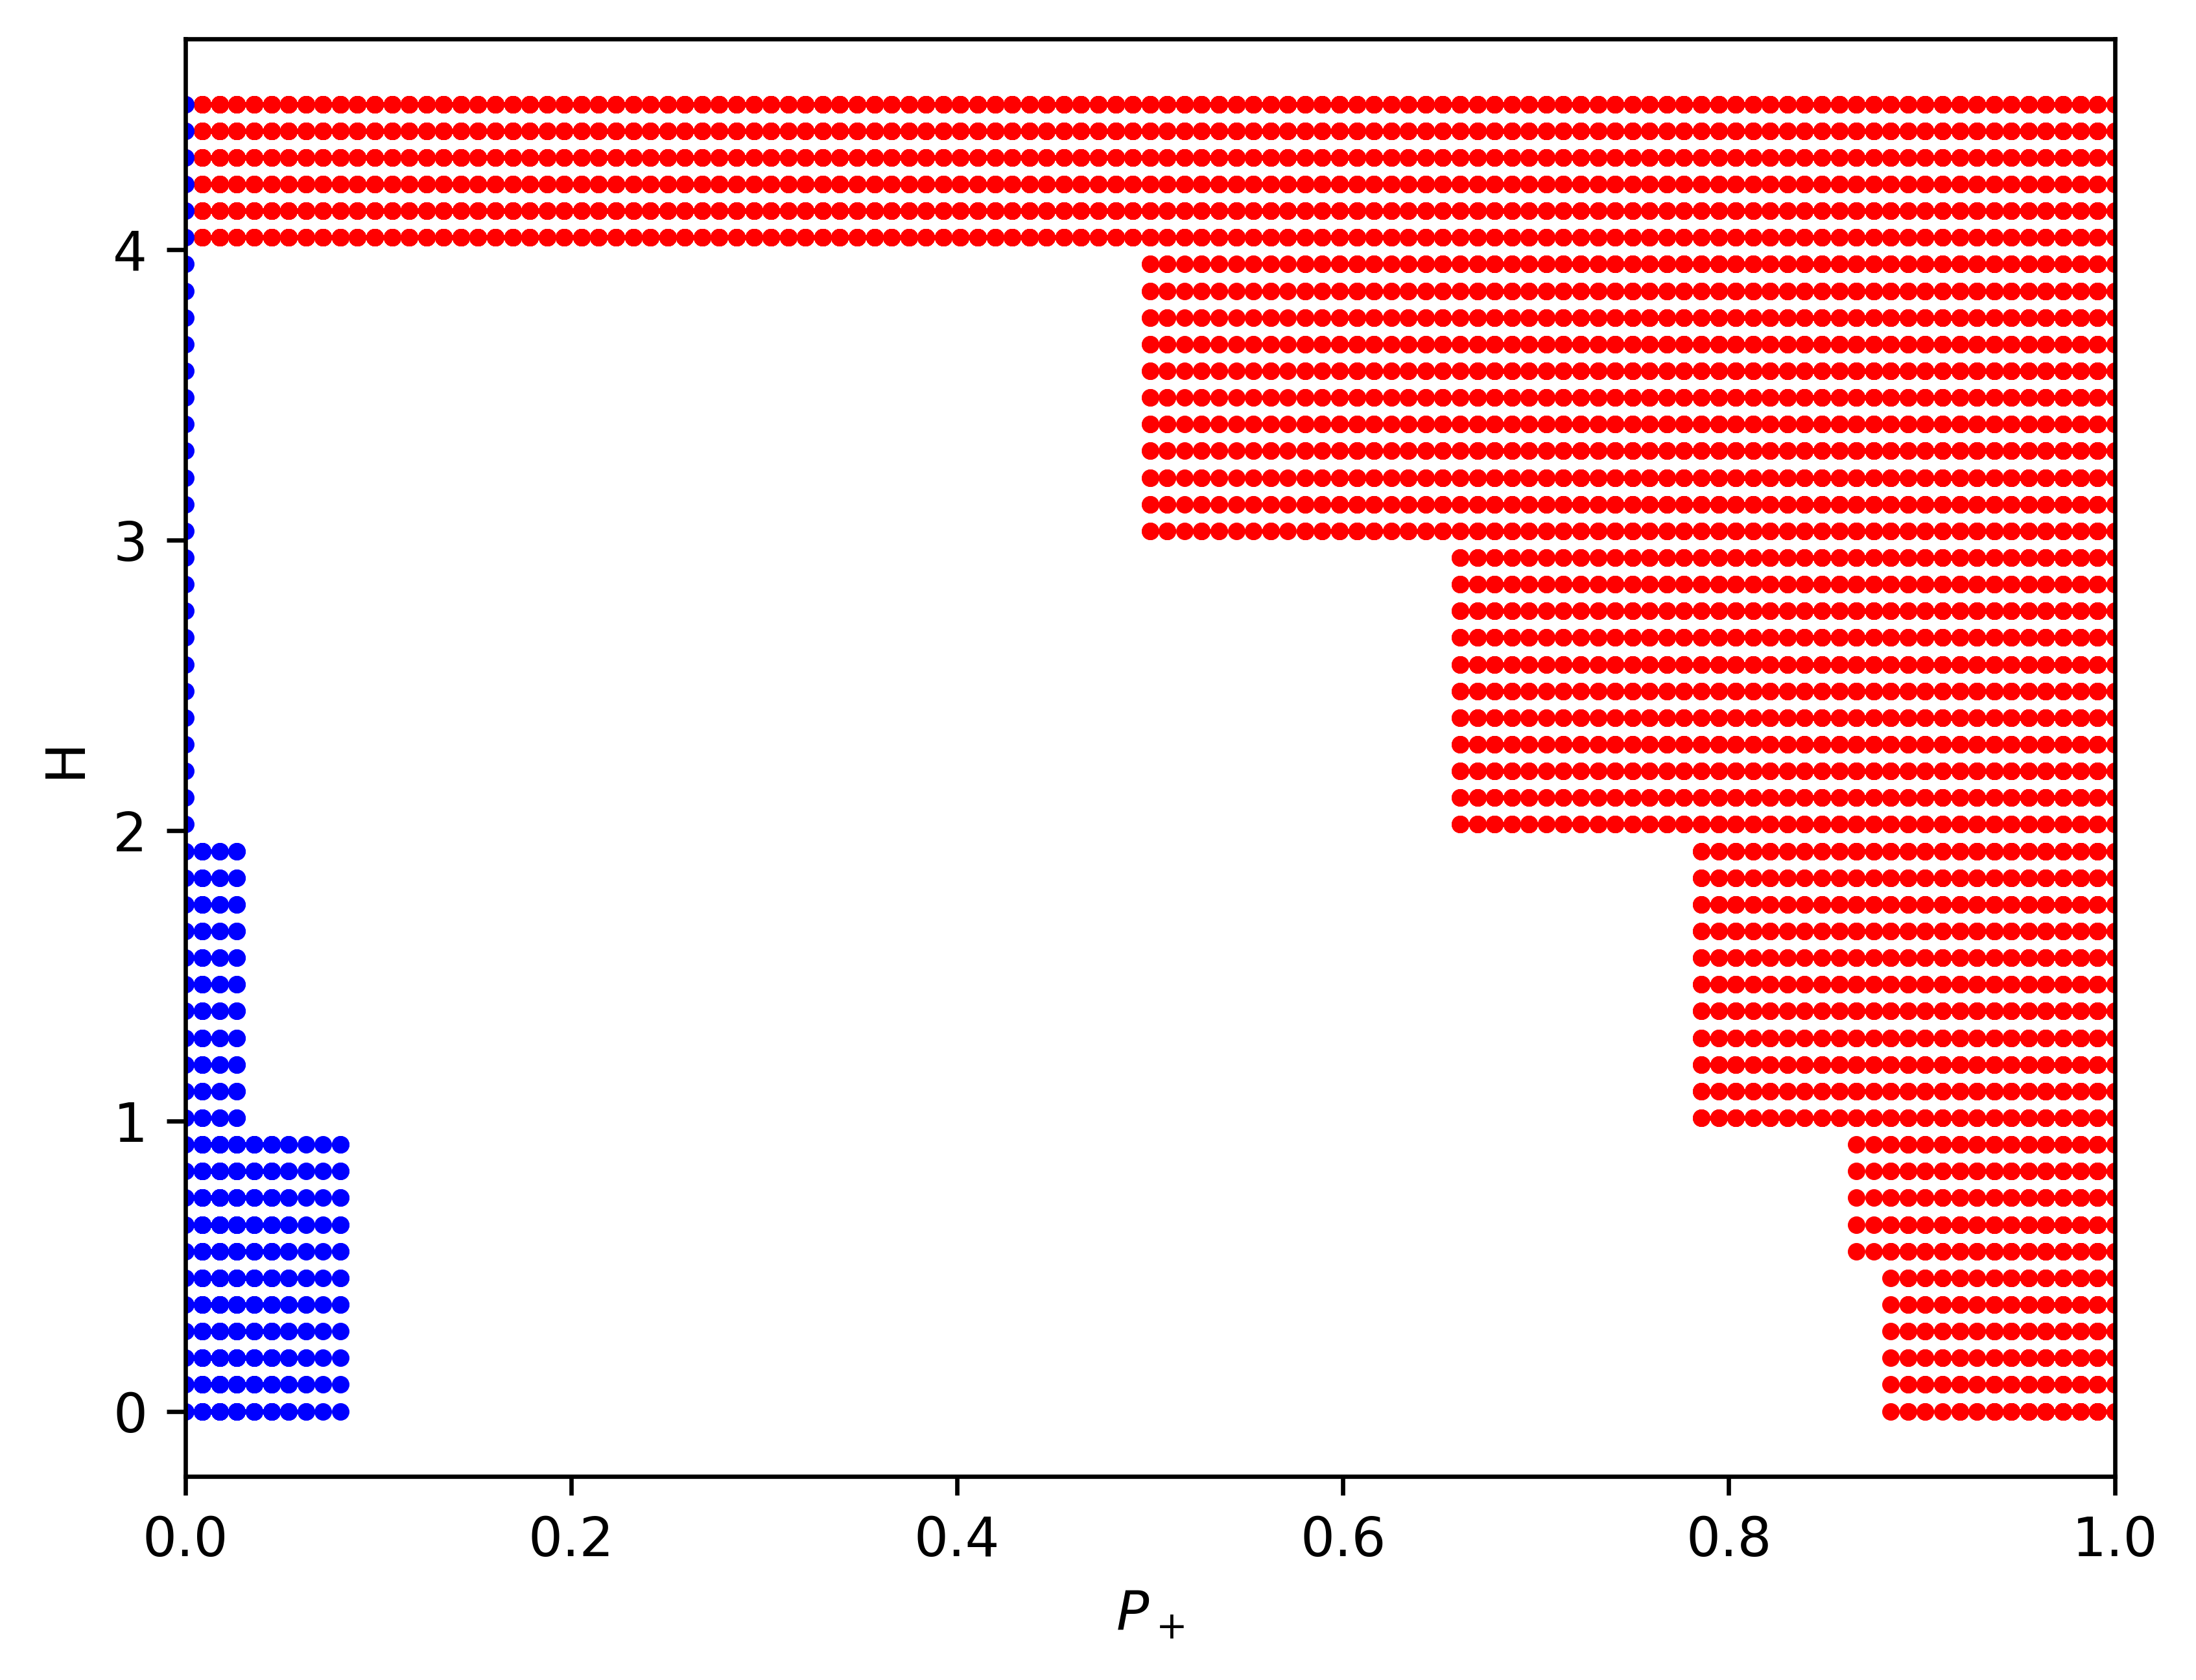
\includegraphics[width=0.8\textwidth]{images/P+_afm_fm(H)_filled.png}
	\caption{Approximate phase separation at $T = 0$ in an external magnetic field. Blue dots: antiferromagnetic phase; red dots: ferromagnetic phase}
	\label{fig:P+_afm_fm(H)}
\end{figure}

Applying an external magnetic field shifts phase boundaries. For $h/J > 1$, a spin-flop transition occurs in some samples, and for $h/J > 2$, it occurs in all. At $h/J > 4$, all samples transition to a ferromagnetic state.

The staircase-like behavior of the diagram can be explained by the competition between internal interaction energy ($E = -\sum J_{ij} S_i S_j$) and Zeeman energy ($E = - h \sum S_i$). At specific field values, the Zeeman energy dominates, causing phase transitions across groups of samples with varying $P_+$.

It should be noted that open boundary conditions may introduce significant distortions. For example, a sample with $P_+ = 0.2$ (Figures \ref{fig:Mgs(P+)} and \ref{fig:P_AFM_FM_Mmax}) exhibits antiferromagnetic properties due to ferromagnetic bonds ($J_{ij} = 1$) being concentrated along the edges.

\section{Conclusion}

An exact solution for the ground state of the Edwards-Anderson model on a simple square lattice of $8 \times 8$ spins has been obtained and analyzed using an complete enumeration method. The developed algorithm enables calculation of degeneracy, energy, and spin excess for each of the $2^N$ possible states, facilitating studies at zero temperature and in the presence of a nonzero external magnetic field $h/J$.

It has been demonstrated that the macroscopic degeneracy of the ground state in finite-sized frustrated spin systems within the Edwards-Anderson model is governed by the combinatorics of frustrated plaquettes, i.e., the number of ways to arrange frustrated spin pairs on the lattice. An algorithm has been proposed for calculating energy, spin excess, and ground-state configurations based on the determination of frustration locations. The algorithm is limited by the number of possible arrangements of frustrations.

It was established that Type-II plaquettes are the sole source of frustration in the ground state in the absence of an external magnetic field. In energy-minimizing configurations, frustrations may also appear between Type-II plaquettes or between a frustrated plaquette and the lattice boundary, depending on the distances and boundary conditions. Macroscopic ground-state degeneracy implies alternative arrangements of frustrations.

The dependence of the ground-state spin excess in the Edwards-Anderson model on the external magnetic field at $T \to 0$ exhibits a discrete (stepped, staircase-like) character. This behavior is caused by the discrete structure of the density of states. Critical values of the external magnetic field, where giant jumps in residual entropy are observed, have been calculated. The nature of these entropy jumps arises from the fact that at certain critical field values, multiple spin configurations with different interaction and Zeeman energies—but the same total energy—contribute equally to the ground state. Degeneracies of states with identical total energy are summed.

The problem of the maximum number of frustrations as a function of the number of spins in a system for a given lattice type in the Ising model with antiferromagnetic and ferromagnetic exchange interactions is of interest, as the presence of frustrations gives rise to new properties. It has been shown that in the Edwards-Anderson model, systems with twofold ground-state degeneracy can exist, and configurations of minimum energy may include frustrations. Additionally, the placement of frustrations in ground-state configurations (i.e., the degeneracy of states with nonzero spin excess) and the suppression of frustrations by an external magnetic field could be subjects of further research.


\section{Acknowledgments}

The research was supported by the Russian Science Foundation grant No. 24-71-10069, https://rscf.ru/en/project/24-71-10069/.

\bibliography{mybibfile}


\end{document}